\documentclass[sigconf,nonacm]{acmart}
\usepackage{amsmath,amssymb,amsthm}
\usepackage{booktabs}
\usepackage{graphicx}
\usepackage{xcolor}
\usepackage{array}
\usepackage{balance}
\usepackage{tikz}
\usetikzlibrary{arrows.meta,positioning,fit,backgrounds}
\usepackage{lmodern}

\newcommand{\tab}{Table~}
\newcommand{\fig}{Figure~}
\newcommand{\thm}{Theorem~}
\newcommand{\cor}{Corollary~}
\newcommand{\us}{\ensuremath{\,\mu}s}
\newcommand{\code}[1]{\texttt{\detokenize{#1}}}
\newcommand{\eq}{Equation~}
\newcommand{\mth}[1]{\ensuremath{#1}}
\newcommand{\ms}{ms}

\newtheorem{theorem}{Theorem}
\newtheorem{lemma}[theorem]{Lemma}
\newtheorem{corollary}[theorem]{Corollary}
\theoremstyle{definition}
\newtheorem{definition}[theorem]{Definition}
\newtheorem{assumption}[theorem]{Assumption}

\newcommand{\B}{B}
\newcommand{\Lam}{\lambda}

\setlength{\emergencystretch}{3em}
\begin{document}

\title{Bounded Reclamation: Compile-Time Tiering, Pause and Memory Contracts,\ and a Roofline for Reclamation Policy}

\author{The extC Project}
\affiliation{\institution{extC Compiler Project}\country{China}}

\begin{abstract}
A managed run-time owes its users two numbers it rarely states: how much memory it will use, and how long it may pause.
Collectors answer neither, because a collector is a scheduler: it decides at run time when to work, how much to work, and how long the mutator waits.
This paper describes extC, a systems language whose reclamation is decided entirely at compile time and whose run-time work is a bounded, incremental algorithm, and it turns the two numbers into contracts that can be checked.

Three ideas carry the design.
First, the compiler places every allocation in one of five storage substrates --- frame arenas, typed reclamation regions, container pools, per-task arenas, and address-reserved plates --- so that four of the five have a scope-derived lifetime and need no collector at all.
Second, for the one substrate that can hold cycles the compiler emits one of three tiers per translation unit: no reclamation code at all (544 of the 794 corpus programs that compile, 68.5\%), an event tier that counts and never sweeps, or an incremental mark-and-sweep tier whose work is cut into segments by a wall-clock deadline, charged against an allocation quota, and whose region destruction is deferred through an $O(1)$ closing queue.
Third, every run-time decision that could grow without bound is given a budget and a proof: the pause of one step is bounded by a segment length, the heap is bounded by the live set through a trigger law, and the admission of an allocation reserves room for the largest request so that a single object can never overrun the wall.

We prove the safety of the scheme (no dangling reference) together with tier soundness, idle transparency, bounded memory, bounded pause, amortized work, and the progress of deferred destruction, and we machine-check the core of the model in Lean~4.
We then formalize reclamation policy as a roofline: the cost per allocated byte is $\lambda(r) = (c_t + c_s F r)/(r-1)$, memory follows $M = L + \kappa_M H$, a step of $b$ pops costs $P(b) = b\tau_t + W_s 64 \tau_s$, and keeping up with the mutator requires $r \ge 1 + gK/b$; the admissible policies form a band on the $(\lambda, a)$ plane whose walls are the memory budget and the pause budget, and the optimal policy sits on both.
All six constants are measured, and the model tracks measurement to within 2--10\%.

On four cross-language workloads extC matches the best Rust arm on promotion (39.0 vs 39.1~ms), beats the best C++ arm on size-ratio (16.0 vs 17.9~ms) and on a ring workload (15.0 vs 36.1~ms), and is within 1.1\% of C++ on a pointer-chasing graph at 13\% lower peak memory, while no workload shows a single pause above one millisecond and the graph shape has a 99.9th-percentile pause of $58\,_\mu$s.
Turning reclamation off makes the allocation-heavy shapes 1.5--3.7 times slower and 17--59 times larger in memory, which is the cost the design removes.

\end{abstract}

\keywords{memory management, region reclamation, escape analysis, compile-time switching, pause bounds, roofline model, formal verification}

\maketitle

\section{Introduction}
\label{sec:intro}

A systems language that manages memory must answer one question before any other:
how does it find the objects that are still in use?
Tracing collectors answer with the program roots, which requires a run-time that can scan stacks and registers,
a dedicated thread or at least a stop-the-world rendezvous, and a representation in which the collector can tell a pointer from an integer.
Reference counting answers with the store itself, which requires a barrier on every pointer write and leaves cycles uncollected.
Both answers are structurally expensive: the first builds machinery that suspends or schedules across the whole program,
the second puts the machinery on the hottest path in the program even when almost nothing is shared.

This paper starts from a different observation.
Most functions in a managed program never create, overwrite, or drop a reference that outlives the function.
That is not an approximation to be measured at run time, it is a property to be proved at compile time.
When the proof holds, the compiler can emit code that frees memory at the end of the owning block and nothing else,
and the whole reclamation run-time can be absent from that function.
extC, a small systems language that compiles to C and checks view lifetimes with a depth-indexed escape analysis,
uses this observation as its organizing principle: the compiler derives the root set statically, decides per translation unit
which of three reclamation tiers to emit, and, where a run-time is emitted, gives every unit of its work a budget.

\noindent\emph{From a mechanism to a contract.}
Being able to switch the run-time off is a qualitative result; it is not yet a promise a latency-sensitive user can sign.
What such a user needs is two numbers: an upper bound on the heap and an upper bound on the pause. Our earlier design
reported a pause \emph{distribution}, which is the wrong object to promise, because a distribution has a tail and the tail is
what the user feels. This paper therefore restates the design as a set of contracts and then proves them:
every step of reclamation work has a work bound that does not depend on the size of the heap or of a region;
the heap obeys a trigger law that ties its peak to the live set; the destruction of a whole frame is deferred through an
$O(1)$ queue so that no single step can pay for the frame; and the admission of an allocation reserves room for the largest
request, so that a single large object cannot overrun the wall between one collection and the next.

\noindent\emph{What the compiler computes.}
The compiler assigns each allocation site to one of five storage substrates: a frame arena, a typed reclamation region,
a container pool, a per-task arena, or a plate from \texttt{std.mem}.
Only the reclamation region needs a collector.
Reference objects that can escape to the function level go there, in a non-moving, non-stop-the-world, incremental
mark-and-sweep over typed slabs whose roots are emitted statically; everything else is freed by dropping its scope.
For the reclamation region, a unit-level proof decides the tier: if no function in the unit needs any reclamation work,
nothing is emitted; if the unit is proved acyclic under a single-level-churn condition, counting is emitted and sweeping is
not; otherwise the mark-and-sweep tier is emitted with counting compiled out.

\noindent\emph{Why a roofline.}
Tuning a reclamation policy has four knobs (the trigger ratio, the batch size of a step, the segment length, and the
reclamation credit) and two hard constraints (memory and pause), and practitioners tune it by folklore.
We show that the trade-off has the shape of a roofline model, in the same sense as the GPU model of attainable
performance: the analogue of arithmetic intensity is the reclamation cost per allocated byte, $\lambda$, and the analogue of
attainable throughput is the allocation rate the mutator reaches once reclamation work is charged to it.
The cost of a round is mark plus sweep, the memory is live set plus a fraction of the trigger, and the keep-up condition
is a lower bound on the trigger ratio. These three laws carve an admissible band out of the plane, and within that band the
optimal policy is the one that pushes both knobs to their walls --- more precisely, to the memory wall and the pause wall.
The model is calibrated with six constants measured on the implementation, and it predicts the measured cost of a round to
within a few percent.

\noindent\emph{Results.}
We evaluate on four workload shapes that isolate promotion, size turnover, pointer chasing, and ring turnover, against nine
arms of C++, Rust, Go, Java and JavaScript built from the same specification, in one interleaved frozen run that also checks
that every arm prints the same answer (Section~\ref{sec:eval}).
extC matches the fastest Rust arm on the promotion shape (39.0 against 39.1~ms), is faster than the best C++ arm on size
turnover (16.0 against 17.9~ms) and on the ring (15.0 against 36.1~ms), and is 1.1\% slower than C++ on pointer chasing while
holding 13\% less peak memory.
No shape shows a single pause above one millisecond; the 99.9th percentile is $10$--$58\,_\mu$s depending on the shape, and the
shape that pauses longest is the one with the largest live set, not the one that allocates most.
Turning reclamation off instead of on is not a free lunch: the allocation-heavy shapes become 1.5--3.7 times slower and
17--59 times larger, because reclamation replaces page faults with reuse.
A mechanism ablation that recompiles the same generated program with one budget changed at a time (ten variants) shows which
constant buys what, and where a choice went against us --- a larger scan chunk, a smaller slab, a padded slot --- the measurement
says so and the design keeps the version that survives it.

\noindent\emph{Contributions.}
\begin{itemize}
\item A description of extC memory management as five substrates and a three-tier compile-time switch, with the exact
  static conditions under which each tier is emitted, and a census of every \texttt{.extc} file in the tree showing that
  68.5\% of the programs that compile need no reclamation run-time at all.
\item A soundness theorem for the full current scheme (no dangling reference) that covers, in addition to the four layers of
  the earlier design, the deferred destruction of regions through the closing queue, the reservation made by admission, and
  the switch between tiers.
\item A bounded-pause theorem: one step of marking walks at most a segment or a wall-clock deadline, one step of sweeping
  releases at most a credit, one step of deferred destruction moves at most a fixed number of slabs, and the sum is bounded
  by constants that do not depend on the heap or on the region.
\item A roofline model of reclamation policy: a cost law, a memory law, a pause law and a keep-up law, an admissibility
  theorem that reduces to one inequality, an optimality theorem that puts the optimum on both walls, and a Pareto frontier;
  six calibrated constants and a validation against measurement.
\item A machine-checked core: 13 Lean~4 modules with no \texttt{sorry} covering region safety, the reclaim rule, the idle
  analysis optimality, and the memory-gap law, with a table mapping each paper theorem to its machine-checked counterpart and
  an explicit statement of what the machine check does not cover.
\item An evaluation from one frozen interleaved run: nine arms over four shapes across six languages, a ten-variant mechanism
  ablation, pause distributions with the total work share, a boundedness experiment that scales the round count by $8\times$,
  code-size measurements, and a census.
\end{itemize}


\noindent\emph{Roadmap.}
Section~\ref{sec:design} describes the design operationally, Section~\ref{sec:formal} states the calculus and the theorems,
Section~\ref{sec:roofline} derives the roofline model, Section~\ref{sec:impl} maps the design onto the compiler, and
Section~\ref{sec:eval} measures it. Section~\ref{sec:limitations} states where the design does not apply.

\section{Design}
\label{sec:design}

extC keeps the part of a C-like language that makes memory behaviour predictable:
objects never move, layouts are deterministic (there is no object header, and no word of a value
is ever reserved for the runtime), and there are no write barriers on data stores.
The design question we answer here is how reclamation fits into that shape without giving up
bounded memory or bounded pause.

Our answer has three parts.
(1) \emph{Storage is stratified by lexical scope.} Every allocation point has a statically known
level, and the level selects one of five substrates (\S\
ef{sec:substrates}), each with a different
reclamation rule.
(2) \emph{Reclamation is a compile-time decision.} A unit is analysed and placed in one of three
tiers (\S\
ef{sec:tiers}): no runtime at all, an event tier where reference counts free objects on
the spot, or a sweep tier where each region is marked and swept under explicit budgets.
(3) \emph{The runtime obeys a two-dimensional contract.} Memory is bounded by a wall that the
collector's trigger line respects, and each synchronous step of the collector is bounded by a
budget that is independent of the heap size (\S\
ef{sec:contract}).

\begin{table}[t]
\centering
\small
\begin{tabular}{@{}p{0.15\linewidth}p{0.19\linewidth}p{0.26\linewidth}p{0.28\linewidth}@{}}
\toprule
Substrate & Lifetime owner & Allocation & Reclamation \\
\midrule
Frame arena & lexical scope of a block & bump pointer in a chunked arena & whole arena rewound on scope exit \\
RC region & frame level (a function or block) & slot in a slab, size class by request & budgeted mark--sweep inside the region \\
Pool & the \texttt{place} the container was created in & slab chain rooted at that place & chain rewound with the place \\
Task arena & coroutine frame or parallel worker & bump, thread-local & arena discarded when the task ends \\
Plate & explicit \texttt{plate} value, OS pages & \texttt{mmap} of page-rounded bytes & \texttt{mprotect} / \texttt{munmap} \\
\bottomrule
\end{tabular}
\caption{The five storage substrates. Only the third row is managed by the reclamation runtime;
the others are released wholesale, so their cost is paid once per scope or per task.}
\label{tab:substrates}
\end{table}

\subsection{Storage substrates}
\label{sec:substrates}

\tab\ref{tab:substrates} lists the substrates.
Which one a \texttt{new} lands on is decided by the level of its frame, not by its type, so the
same struct can be arena-allocated in one place and region-allocated in another.

\paragraph{Frame arenas.}
A block that is not a reclamation region gets a bump arena: a chunk list whose allocation is one
pointer increment, and whose exit restores the pointer to the block entry.
The zero cost of this row is what the whole design is trying to preserve, and \S\
ef{sec:eval}
shows that 71.7\% of the compiling programs in our corpus still get it for free (\S\
ef{sec:census}).

\paragraph{Reclamation regions.}
A region is a set of slabs owned by one frame level.
Each object occupies exactly one slot; the slot stride is the request rounded up to a multiple of
eight, so an 80-byte object occupies 80 bytes rather than the next power of two.
Per-slot metadata is kept in three bitmaps (occupied, marked, cross-region registration) plus a
16-bit type number and a 16-bit in-edge count, so the payload is byte-exact and the layout of a
value is never perturbed by the runtime (\S\
ef{sec:impl-geometry}).

\paragraph{Pools and plates.}
Containers whose element type is known allocate from a slab chain attached to the \emph{place}
where they were created, so a container that dies with a block releases its storage with that
block instead of being swept.
Plates are the escape hatch for data that must outlive the process's own structure: page-aligned
\texttt{mmap}, optionally protected, released explicitly.

\paragraph{Task arenas.}
A coroutine frame and a parallel worker each get a thread-local arena that is discarded when the
task ends (\texttt{extc\_par\_close} for workers, frame teardown for coroutines).
Freshly spawned tasks that write into their owner's view get references pinned to the owner's
region instead, so a task can never leave a dangling edge behind when it is torn down.

\subsection{Placement and escape}
\label{sec:placement}

Levels are assigned by the escape analysis: parameters are at level $0$, a function body at
$1$, and each nested block adds one.
An allocation point's region is the level where its storage must live:
\begin{equation}
\ell(pi) = \max(0, k - \mathit{escapeDepth}(pi)),
\label{eq:placement}
\end{equation}
where $k$ is the lexical depth of the allocation point and $escapeDepth$ is the number of
levels the value escapes.
Three rules keep the stratified store sound:

\begin{itemize}
\item \emph{D1 (no downward edge).} Storing a reference into a slot at depth $e$ requires the
  pointed-to storage to be at depth $d \le e$. Storing a younger object into an older slot is
  allowed; the reverse would let a scope outlive its referent.
\item \emph{D2 (promotion is static).} If a value may escape to level $d$, its allocation point
  is placed at level $d$ at compile time: the storage is born there, nothing is copied or moved at
  run time, and the object's address is fixed from birth. The only run-time cost at an escape site
  is the one pointer store that puts the reference into an outer slot.
  Whether a value lives in a long-lived region is therefore known statically, and
  \S\ref{sec:formal} never has to reason about a move.
\item \emph{D3 (views).} A view may not outlive the storage it views: $d \le c$ for view
  $c$ of container $d$.
\end{itemize}

Promotion is where unbounded memory can appear: the storage now lives until the outer level ends,
although only one of the values written into it may still be reachable. That is the shape the
reclamation tier exists for, and the shape \S\
ef{sec:formal} reasons about.

\subsection{Choosing a tier}
\label{sec:tiers}

After placement, the unit is analysed as a whole and assigned a tier.
The assignment is a pure compile-time decision; two user-visible switches
(\texttt{EXTC\_RECLAIM}, \texttt{EXTC\_RC\_SWEEPFREE}) only force or forbid a tier, and they exist
for the experiments in \S\
ef{sec:eval}.

\paragraph{Tier 0: no runtime.}
If no allocation point is governed by reclamation, the emitted program contains no reclamation call
and the runtime text is not even emitted (a 434-line \texttt{hello} world has zero
\texttt{extc\_rc\_} tokens). This is the default outcome for programs that never promote.

\paragraph{Idle units.}
A unit is \emph{idle} when every reference field is written at most once per object, no reference
local or parameter is reassigned in a way that drops a reference, and no operation drops a
reference (\S\
ef{sec:formal-idle} formalises this).
An idle unit needs no reclamation work at all: objects only disappear when their whole region is
released. The judgement is conservative and whole-unit, so one function that fails it keeps the
runtime for the unit.

\paragraph{The event tier (T1).}
The event tier is taken when the unit is \emph{acyclic}: every reference write either stores a
freshly allocated value, \texttt{null}, or a value from a strictly older level, and every slot that
can drop a reference is a counted slot.
Under those conditions no cycle can form and every object that becomes unreachable reaches count
zero, so the runtime keeps reference counting and does not emit sweeping.

\paragraph{The sweep tier (T2).}
Otherwise the unit gets cyclic-capable regions: counting is off by default (the
\emph{no-count} configuration) and unreachable storage is recovered by budgeted mark--sweep over one
region at a time.
Counting is not needed for safety in this tier -- the marker finds its seeds from the static root
table and the cross-region registration bits, not from counts -- so switching it off only removes a
fast path, never a guarantee.

\begin{table*}[t]
\centering
\small
\resizebox{\ifdim\width>\linewidth\linewidth\else\width\fi}{!}{\begin{tabular}{@{}llccc@{}}
\toprule
Tier & When & Counting & Sweeping & Contract \\
\midrule
T0 & user forces \texttt{EXTC\_RECLAIM=0} & no & no & memory not bounded (control group) \\
none & $\mathit{idle}(U)$ & no & no & region wholesale release only \\
T1 & $\mathit{acyclic}(U)$ & yes & no & $O(1)$ free, memory $\le L + G + O(B)$ \\
T2 & otherwise & no (default) & yes & budgeted mark--sweep \\
\bottomrule
\end{tabular}}
\caption{Tier assignment. The last two rows are the ones that emit a runtime; T0 and the idle case
emit none. \S\
ef{sec:formal} gives the soundness statement for each row.}
\label{tab:tiers}
\end{table*}

\subsection{The two-dimensional contract}
\label{sec:contract}

Let $L$ be the live set of a region (bytes reachable from a complete root table), $M$ the
bytes the region has ever admitted, and $M_max$ the wall.
Two properties are promised for every program that runs in T1 or T2:

\begin{description}
\item[Bounded memory.] $M \le L + G + O(B)$ where $G$ is the trigger floor and $B$
  the size of one slab, and the bound does not depend on the number of loop iterations, i.e.~it is a
  function of the live set, not of the total allocation volume.
\item[Bounded pause.] Every synchronous step the collector takes on the mutator thread is bounded by
  a constant $P_{\max}$ fixed at compile time, independent of the heap size and of the size of
  the object being scanned. Pause here means the sum of all collector time on that thread, not a
  stop-the-world window: there is no separate collector thread to hide work in.
\end{description}

The contract is maintained by four release layers, each of which removes a different class of
garbage:
\begin{enumerate}
\item \emph{Scope exit} rewinds the arena (zero cost).
\item \emph{Static placement} puts the storage of an escaping value directly at the level it
  escapes to; at run time an escape costs one pointer store, never a copy.
\item \emph{Count zero} frees exactly one object at the moment its last holder drops it (T1, and
  optionally T2).
\item \emph{Region sweep} recovers what the first three cannot: cycles, and storage whose counts were
  saturated deliberately.
\end{enumerate}

Counting is a knob, not a guarantee: turning it off changes which layer reclaims a given object, not
whether the program is safe, and the sweep tier therefore stays correct with counting disabled.

\subsection{Deliberate non-goals}
\label{sec:non-goals}

We do not move objects, so no compaction and no copying collection: fragmentation is bounded by the
size-class layout, not eliminated.
We do not scan stacks: the root table is static, emitted at each trigger point, which is why the
collector needs no shadow stack and why a suspended coroutine registers its frame fields instead.
We do not run the collector on another thread, so \emph{every} collector instruction is mutator time;
this is the honest reading of our pause numbers and the reason \S\
ef{sec:eval} reports both the
armed-window total and the per-step total.
We do not attempt to bound the pause of a program that allocates an object larger than the wall in a
single request: the admission rule (\S\
ef{sec:impl-admission}) reserves room for one maximum-sized
request, so such a program is rejected by the bound rather than silently breaking it.

\begin{table*}[t]
\centering
\small
\resizebox{\ifdim\width>\linewidth\linewidth\else\width\fi}{!}{\begin{tabular}{@{}lll@{}}
\toprule
Property & Status & Mechanism or reason \\
\midrule
peak memory & bounded by $L+G+O(B)$ & trigger line $\ge 2L$, wall $M_{\max}$ \\
per-step collector time & bounded & batch cap 256, segment deadline 40\,\us \\
region destruction & $O(1)$ & closing queue drained at allocation points \\
one request larger than wall & reserved & admission: $\mathit{thr} + R_{\max} \le M_{\max}$ \\
long-lived garbage in a region & bounded, not zero & sweep is triggered by pressure, not by time \\
count saturation & not a leak & saturated slots stay countable-by-sweep \\
pause of a single huge scan & bounded & object scan chunked into 512-word segments \\
\bottomrule
\end{tabular}}
\caption{What the current design does and does not bound. Each bounded row is backed by a theorem
in \S\
ef{sec:formal} or by a measured gate in \S\
ef{sec:eval}.}
\label{tab:bounded}
\end{table*}
\section{A core calculus, and what it buys}
\label{sec:formal}

\S\ref{sec:design} was operational, because that is how the system is built.
This section states the same design as a small calculus, so that the claims the mechanism rests on
become theorems rather than assertions: a freed slot is never dereferenced (\S\ref{sec:thm-safe}),
a compile-time tier switch is sound (\S\ref{sec:thm-tier}), removing collection work from an idle
function is observationally transparent (\S\ref{sec:thm-idle}), peak memory is a function of the live
set and not of the run length (\S\ref{sec:thm-bounds}), every synchronous collector step has a bound
that is independent of the heap (\S\ref{sec:thm-bounds}), total traversal work is linear in allocated
bytes (\S\ref{sec:thm-bounds}), and deferred freeing still makes progress
(\S\ref{sec:thm-bounds}).

Section~\ref{sec:formal-status} states exactly what is proved here, what is machine-checked in Lean,
what is checked by the compiler's own gates, and what is only tested.

\subsection{Store, frames, regions}
\label{sec:machine}

\emph{Frames} form a stack $F_0, \dots, F_n$ with $F_0$ outermost.
Each frame owns \emph{regions}, written $\rho^{\ell}$ where $\ell$ is the frame's distance from the
ground ($\rho^{0}$ belongs to $F_0$ and lives longest).
We use one direction throughout: \emph{smaller $\ell$ is longer-lived}.

A region is a sequence of \emph{slabs}; a slab is partitioned into \emph{slots}; a slot holds
either scalars, a struct, a \emph{view} $(p, \mathit{len})$, or a \emph{reference} $p$.
Every slot $\sigma$ has a type descriptor $\delta(\sigma)$ naming its reference words, and a
\emph{status} $\mathit{st}(\sigma) \in \{\mathsf{live}, \mathsf{free}\}$; the status of slots in a
released region is $\mathsf{free}$ and its memory is returned to the allocator.

Runtime state is a pair $(M, \mathit{sh})$ of a memory $M$ mapping slots to values and a shade set
$\mathit{sh}$ used by the incremental marker.
$\mathit{reach}_M(S)$ is the set of slots reachable from $S$ by following references and views
through the type descriptor of each slot; $\mathit{root}(F) = R(F)$ is the frame's \emph{root table},
a static list of the slots named by its reference-typed locals and parameters, emitted with the code
of $F$ and never computed at run time.
$\mathit{seeds}(\rho) = \bigcup_F R(F) \cup \mathit{foreign}(\rho)$ is the seed set of a region,
where $\mathit{foreign}(\rho)$ is the set of slots in $\rho$ that other regions register as
cross-region entry points.

\subsection{Static judgments}
\label{sec:judgments}

\paragraph{Placement.}
For an allocation site $s$ at depth $k$ the analysis yields a level
$\ell(s) = \max(0, k - \mathit{escapeDepth}(s))$ (eq.~\ref{eq:placement}) and the site allocates
directly in $\rho^{\ell(s)}$.
Nothing is moved later: there is no promotion copy at run time.

\paragraph{Depth rules.}
Every local, parameter and slot carries a \emph{depth} $d$ (the level of the region that holds it,
on the same scale; smaller is longer-lived):
\begin{enumerate}
\item[(D1)] a reference may be stored into a slot of depth $e$ only if the storage it names has
  depth $d \le e$;
\item[(D2)] if a value may escape $j$ frames, its site is placed at $k - j$, so at every escape site
  the reference is stored into a slot no shallower than the storage it names -- the store is one
  word write, and there is no copy of the value;
\item[(D3)] a view of container depth $d$ may only be used in a context whose depth $c$ satisfies
  $d \le c$.
\end{enumerate}
Violating (D1)--(D3) is a compile error, not a runtime check.
Two mutable references may alias and values are copied by default; no rule assumes uniqueness.

\paragraph{Tier judgments.}
$\mathit{acyclic}(U)$ holds when every reference write in $U$ either (i) stores a value freshly
allocated in the same frame, or a call result proved acyclic and fresh, (ii) stores \texttt{null},
(iii) stores a value from a strictly older level, or (iv) is a counted slot, and no other write can
drop a reference (this is the checker's \texttt{planFnAcyclic} condition, applied to every function
of the unit).
$\mathit{idle}(U)$ holds when every reference field is written at most once per object, no reference
local or parameter is reassigned in a way that drops a reference, and no operation drops a reference;
a call to a non-idle callee counts as a drop.

\subsection{Runtime transitions}
\label{sec:transitions}

The mechanisms of \S\ref{sec:contract} are transitions on $(M, \mathit{sh}, q, \mathcal{S})$,
where $q$ is the closing queue and $\mathcal{S}$ the free queue.
Write $\mathit{free}(\rho, S)$ for freeing the slots $S$ of $\rho$, and
$\mathit{live}(M) = \mathit{reach}_M(\bigcup_F R(F))$.

\begin{description}
\item[Allocate.] Take a free slot of the right size class (or bump a slab), set it $\mathsf{live}$,
  zero it, and if a mark round is in flight mark it black.
\item[Field store.] Write a value; if a mark round is in flight, shade the new value (insertion
  barrier) and, when replacing a reference, shade the old one (deletion barrier).
\item[Local release.] On block exit, the block's arena is rewound whole.
\item[Count zero.] A reference-counted slot whose count reaches zero is freed on the spot.
\item[Mark step.] Pop at most $b$ objects from the mark stack, scan each through its descriptor, and
  resume one chunked object scan if one is in progress; at most $\mathit{CHUNK}$ words of a resumed
  scan are visited before the cursor is saved again.
\item[Sweep step.] Visit at most $W_s$ words of a region's occupancy bitmap and free the slots of
  dead words.
\item[Trial delete.] On an overwrite that satisfies the four static conditions of \S\ref{sec:design},
  mark from $\mathit{seeds}(\rho) \setminus \{\sigma\}$ and free the slots reachable from the old
  value but unreachable from the remaining seeds.
\item[Close.] On region death: abort an in-flight round, drop the region's pins, set
  $\mathit{dead}(\rho)$, and append $\rho$ to $q$; this part is $O(1)$.
\item[Drain closing.] At an allocation point, pop regions from $q$, unlink their slots'
  cross-region edges, remove their registry entries, and push their slabs to $\mathcal{S}$;
  bounded by $\mathit{SLABS}$ slabs or $\mathit{D}_{	ext{cq}}$ microseconds per step.
\item[Drain free queue.] Return at most $\mathit{SLABS}$ queued slabs to the allocator, or stop at
  $\mathit{D}_{	ext{fq}}$ microseconds.
\item[Admit.] Before allocating $n$ bytes, if the next allocation would cross the trigger line, run
  the collector; under an explicit wall the trigger line satisfies $\mathit{thr} + R_{\max} \le M_{\max}$,
  so a request of size at most $R_{\max}$ always fits.
\end{description}

\subsection{Invariants and safety}
\label{sec:thm-safe}

\begin{description}
\item[(I1) Root completeness.] At every trigger point, $R(F)$ contains every live reference slot of
  $F$; for a region handed to the sweep, $\mathit{seeds}(\rho)$ contains every entry into $\rho$ from
  outside.
\item[(I2) Live references name live storage.] If $\sigma$ is live and its reference word holds a
  pointer to $\sigma'$, then $\sigma'$ is live.
\item[(I3) No live reference names freed storage.]
\item[(I4) Dead regions are unreachable.] After $\mathit{dead}(\rho)$ is set, no live slot and no
  seed names a slot of $\rho$.
\end{description}

\begin{assumption}[Escape and root soundness]
\label{as:sound}
(i) the placement and depth rules are enforced; (ii) at every trigger point the emitted root table
is complete in the sense of (I1); (iii) type descriptors list exactly the reference words of a layout;
(iv) C externs never write a reference word of a region slot.
\end{assumption}

\begin{lemma}[Local release is safe]
\label{lem:local}
Freeing a block's arena cannot free storage named by a live reference.
\end{lemma}
\begin{proof}
By (D1), a reference stored outside the block has depth at most the block's depth, so the object it
names has depth at most that too -- it is in this arena or a deeper one, all of which are released no
later. Hence no slot released here is named from an outer, still-live slot.
\end{proof}

\begin{lemma}[Sweep only frees unreachable slots]
\label{lem:sweep}
Under (I1), $\rho \setminus \mathit{reach}_M(\mathit{seeds}(\rho)) \subseteq
\bigcup_{\sigma \in \rho} \{\sigma \mid \text{unreachable}\}$.
\end{lemma}
\begin{proof}
$\mathit{live}(M)$ is reachable from the union of the frames' root tables, and by (I1) every entry into
$\rho$ from outside is in $\mathit{seeds}(\rho)$. A slot in $\rho$ that is reachable from a root is
therefore reachable from $\mathit{seeds}(\rho)$: take the last step of a path before it enters $\rho$
-- that step enters through an entry in the seed set. So the complement of the reachable set inside
$\rho$ is unreachable.
\end{proof}

\begin{lemma}[Trial deletion is conservative]
\label{lem:trial}
The set freed by a trial delete is a subset of the set a full sweep of $\rho$ with the same seeds
would free.
\end{lemma}
\begin{proof}
Trial deletion marks from the same seed set with $\sigma$ removed, so its reachable set is a superset
of the full sweep's reachable set; the freed set is the old value's reachable set minus a superset,
hence smaller. Removing $\sigma$ from the seeds is sound because $\sigma$ holds the old value at that
moment: including it would make the old structure its own justification.
\end{proof}

\begin{lemma}[Deferred region death keeps (I4)]
\label{lem:defer}
Setting $\mathit{dead}(\rho)$ at the owner frame's exit preserves (I2) and (I3), and makes
$\mathit{owns}(p) = 0$ for every $p \in \rho$.
\end{lemma}
\begin{proof}
At the exit of $F$, the only frames that may hold references into $\rho^{\ell}$ are $F$ and deeper
frames; the deeper ones have already exited, and their arenas are gone, so every remaining reference
into $\rho$ lives in $\rho$ itself (or in another region that is dying with the same frame).
Therefore no live slot names $\rho$, i.e. (I3) holds for it, and answering $0$ from
$\mathit{owns}$ cannot hide a live edge: any query that reaches a slot of $\rho$ started from dead
storage.
\end{proof}

\begin{theorem}[No dangling reference]
\label{thm:safe}
Under Assumption~\ref{as:sound}, no execution dereferences a freed slot.
\end{theorem}
\begin{proof}[Proof sketch]
Maintain (I1)--(I4) over the transitions of \S\ref{sec:transitions}.
(I1) is preserved by allocation (the allocating frame records the slot), by the store rule (a
reference stored into a slot of the current frame is a root, and a slot registered from another
region is a foreign seed), and by the fact that roots are only dropped together with the storage that
held them.
(I2) is preserved by allocate, store (the stored value is live by the induction hypothesis) and by
every rule that frees storage: local release (Lemma~\ref{lem:local}), sweep
(Lemma~\ref{lem:sweep}), trial delete (Lemma~\ref{lem:trial}).
(I3) is preserved by those lemmas plus deferred death (Lemma~\ref{lem:defer}), and by the drain
transition, which only unlinks cross-region edges of a region that is already dead.
Dereference is only possible through a reference stored in a live slot, and by (I2) that names a live
slot; a load through a stale pointer copied into a register earlier is excluded by (I3), since the
register contents came from a live slot at the time of the load.
\end{proof}

\subsection{Tier soundness}
\label{sec:thm-tier}

\begin{theorem}[Both tiers are sound, and the switch is a decision]
\label{thm:tier}
Let a unit $U$ be assigned a tier by \S\ref{sec:tiers}.
(a) If $\mathit{acyclic}(U)$, then in the event tier ($T1$) no slot is freed while reachable, and
every unreachable slot is freed within one reference-count update after it becomes unreachable.
(b) If $U$ is placed in the sweep tier ($T2$), then a sweep frees only unreachable slots, whether or
not reference counting is enabled.
\end{theorem}
\begin{proof}[Proof sketch]
(a) The conditions of $\mathit{acyclic}$ make the reference graph a DAG whose edges always point
from a younger (deeper) to an older (shallower) slot, or towards a fresh allocation. Counts
therefore decrease along a topological order: when the last external reference to an object is
dropped, every object reachable only through it has already had its own count reduced to the value
it would have if it were reachable, and a chain of zero counts is freed in one cascade.
No object can be freed while reachable because a reachable object has at least one holder on a live
path, and the cascade only starts from a slot whose count is zero.
The correctness of omitting the sweep is then immediate: the sweep would find every slot reachable
from the seeds, and every unreachable slot has already been freed by counting.
(b) The marker's seed set is the static root table plus the cross-region registration bits; by
Lemma~\ref{lem:sweep} the free set is a subset of the unreachable set. Counts play no role in the
seed construction, so the statement is independent of the \texttt{NOCOUNT} configuration; counting
on only adds the count-zero transition, which is sound by (I2) and can only make the reachable set
smaller.
\end{proof}

\begin{corollary}
\label{cor:tier-switch}
For an acyclic unit, switching the event tier off (forcing $T2$) cannot introduce a dangling
reference; it can only raise the peak memory, because more garbage waits for the sweep.
\end{corollary}

\subsection{Idle transparency}
\label{sec:thm-idle}

\begin{theorem}[Removing collection work from an idle function is transparent]
\label{thm:idle}
If $\mathit{idle}(f)$ holds, then emitting no collection work for $f$ leaves the observable trace of
the program unchanged; only timing changes.
\end{theorem}
\begin{proof}[Proof sketch]
The work emitted for a function is counting updates, budgeted collection steps, root materialization
for callees, and the store barrier.
The idle judgement removes the first three and keeps the barrier: a store an idle function does
perform still shades the edge it deletes, so the tri-colour invariant of the marker is maintained
exactly as in non-idle code.
Two facts are needed. First, a reference stored by an idle function either comes from a slot
reachable at the start of the cycle or is the result of an allocation in the current cycle (black by
construction): the idle conditions forbid reassigning reference locals and forbid writing a
reference field twice in one object, so the value's source is a root or an untouched field.
Second, no slot reachable at entry becomes unreachable during $f$, since $f$ drops no reference.
Hence no omitted step could have been the one that rescues a slot, and the region has the same live
set at exit.
Removing the steps therefore only removes work; induction on the statement structure, with a fixed
point over the call graph, makes the argument well-founded.
\end{proof}

\subsection{Bounds}
\label{sec:thm-bounds}

Let $L$ be the live set at a selection point, $G$ the trigger floor, $B$ the size of one slab and
$\kappa_M$ the measured excess over the live set per unit of retained garbage (the model of
\S\ref{sec:roofline}; $\kappa_M \in [0.772, 1.010]$).

\begin{theorem}[Bounded memory]
\label{thm:mem}
For a loop whose per-round allocation escapes into a bounded set of long-lived slots and whose other
allocations die with the round, the peak of a region satisfies
$M_{\text{peak}} \le L + G + O(B) = L(1 + \kappa_M \cdot r_{\max})$, independent of the number of
rounds, where $r_{\max} = G/L$ is the retention ratio the trigger line allows.
\end{theorem}
\begin{proof}[Proof sketch]
Round-local allocations are released by local release at block exit, so they contribute at most one
round's worth.
A promoted value either lands in a bounded slot set (contributing to $L$) or is overwritten; an
overwritten structure is freed by trial deletion as soon as the credit rule allows a traversal.
The credit rule requires unvisited allocation bytes to exceed $\max(2L, G)$, so between two
traversals the region grows by at most $G$ above its live set, and each denial postpones a free
without stacking: the next round's overwrite makes the older structure unreachable as well, and the
traversal eventually allowed frees the whole chain.
With an explicit wall, the trigger line additionally satisfies
$\mathit{thr} + R_{\max} \le M_{\max}$, so a request up to $R_{\max}$ bytes cannot overshoot the
wall by more than one request, and $R_{\max}$ is itself bounded by the largest single request the
program makes.
\end{proof}

\begin{theorem}[Bounded pause per step]
\label{thm:pause}
Every synchronous collector step performed on the mutator thread finishes in time bounded by
\begin{equation*}
\begin{aligned}
P_{\text{step}} &\le b \cdot \tau_t + \min(C_{\text{scan}}\cdot \mathit{CHUNK},\\
&\qquad D_{\text{seg}} + C_{\text{scan}}\cdot \mathit{CHK}) + W_s \cdot 64 \cdot \tau_s + c_0,
\end{aligned}
\end{equation*}
a constant fixed by compile-time budgets, independent of the heap size, of the number of live
objects, and of the size of the object being scanned; region destruction is $O(1)$ and its deferred
work is charged to the bounded drain steps.
\end{theorem}
\begin{proof}[Proof sketch]
Each step's work item is bounded by construction.
A mark step pops at most $b = \mathit{MARK\_BATCH\_MAX}$ objects and, if an object scan is in
progress, visits at most $\mathit{CHUNK}$ words or stops at the next multiple of
$\mathit{CHK}$ words after the segment deadline $D_{\text{seg}}$; a large object is therefore
scanned across several steps with a saved cursor rather than in one.
A sweep step visits at most $W_s$ bitmap words and frees at most $64 W_s$ slots; the finishing
credit for a slab is clamped by a constant so that the bound does not scale with the slab size.
A trial delete is bounded by the same mark budget because it consumes credit that the credit rule
only grants in proportion to allocated bytes.
Region death does constant work and appends to the closing queue; the queue is drained at
allocation points with at most $\mathit{SLABS}$ slabs or $D_{\text{cq}}$ microseconds per step, and
the free queue likewise.
Summing the bounded terms gives the stated constant; in the measured configuration
$b\cdot\tau_t \approx 4.5$\,\us, $C_{\text{scan}}\cdot\mathit{CHUNK} \approx 8$--$13$\,\us and
$W_s\cdot 64\cdot \tau_s \approx 0.23$\,\us, i.e. a few tens of microseconds per step, which is
what \S\ref{sec:eval} measures.
\end{proof}

\begin{theorem}[Amortized traversal work]
\label{thm:amortized}
Over an execution, the total traversal work charged to a region is
$O(\text{allocated bytes})$ for a region the checker proves acyclic (which additionally never
sweeps), and $O(\text{allocated bytes} + L)$ otherwise; the second bound constrains the total, not a
single step.
\end{theorem}
\begin{proof}[Proof sketch]
For the acyclic case the trigger is never armed with a non-empty mark phase, so the collector is a
no-op and the claim is immediate.
Otherwise each step's work is charged to allocation bytes admitted since the last visit by the credit
rule, and the credit only grows with allocation, so summing over the run gives the bound.
The bound deliberately says nothing about how the work is distributed over the steps; \S\ref{sec:thm-bounds}
supplies that, and \S\ref{sec:eval} measures the distribution.
\end{proof}

\begin{theorem}[Deferred freeing makes progress]
\label{thm:progress}
After a region $\rho$ is closed, the work needed to release it is $O(\text{slabs}(\rho))$, and each
allocation point performs at most $\mathit{SLABS}$ slabs of it, so if the program allocates at all,
$\rho$ is fully released after at most $\lceil \text{slabs}(\rho)/\mathit{SLABS} \rceil$ allocation
points; the closing queue holds at most $\mathit{CQ\_MAX}$ regions, and exceeding that forces an
immediate bounded drain.
\end{theorem}
\begin{proof}[Proof sketch]
Closing does constant work per region and enqueues it.
The drain processes a bounded number of slabs per step and never needs to revisit a slab: unlinking
the cross-region edges of a dead region is a finite walk over its occupied slots, and by
Lemma~\ref{lem:defer} none of those edges can be live.
Since $\mathit{dead}(\rho)$ makes $\mathit{owns}$ answer $0$ for all its slots, the region cannot
acquire new edges while it waits, so the remaining work is monotonically decreasing.
If the program stops allocating entirely before the queue is drained, the remaining slabs are
returned by the process exit path (the OS reclaims them); we state this as an explicit exception
because it is not a bound on the program's own memory.
\end{proof}

\subsection{Status of each claim}
\label{sec:formal-status}

\begin{table*}[t]
\centering
\small
\resizebox{\ifdim\width>\linewidth\linewidth\else\width\fi}{!}{\begin{tabular}{@{}llll@{}}
\toprule
Claim & Paper & Lean~4 & Gate \\
\midrule
Thm.~\ref{thm:safe} safety & proved (sketch + appendix) & \texttt{World.safe\_of\_invariants} & ASan/UBSan corpus \\
Thm.~\ref{thm:tier} tiers & proved (sketch) & \texttt{ExtCRegion}, \texttt{ExtCReclaim} & acyclic/forced red proofs \\
Thm.~\ref{thm:idle} idle & proved (sketch) & \texttt{ExtCIdleMax} (exact) & idle corpus ratchet \\
Thm.~\ref{thm:mem} memory & proved under Assumption~\ref{as:sound} & \texttt{ExtCGap}, \texttt{ExtCMemGap} & boundedness shapes \\
Thm.~\ref{thm:pause} pause & proved by budget counting & \texttt{ExtCPrecision} (footprint per slice) & work-budget gate \\
Thm.~\ref{thm:amortized} cost & proved (sketch) & -- & instruction-count gates \\
Thm.~\ref{thm:progress} deferred free & proved (sketch) & -- & closing-queue driver tests \\
\bottomrule
\end{tabular}}
\caption{What backs each claim. ``Proved'' means the argument in this section; ``Lean'' means the
machine-checked module that covers the corresponding core lemma; ``Gate'' means the automated check
that fails if the implementation stops matching. Blank cells are honest gaps, not claims.}
\label{tab:claims}
\end{table*}

\paragraph{What is assumed.}
Assumption~\ref{as:sound} is the boundary of the whole development.
(i) is the escape analysis, which is a large program that we test and gate but do not prove.
(ii) is what the compiler emits; it is checked structurally by gates that require every trigger point
to materialize the root set the analysis computed.
(iii) and (iv) are checked by construction (descriptors are emitted from the layout) and by the
extern convention (an extern receives references but never writes our slots).

\paragraph{What the Lean development covers.}
Thirteen modules, 2,555 lines, no \texttt{sorry}, checked by \texttt{proofs/verify.sh}: a region
calculus (\texttt{ExtCRegion}, \texttt{ExtCBlock}), the reclamation core
(\texttt{ExtCReclaim}, \texttt{ExtCRuntime}), the gap and memory laws used by
\S\ref{sec:roofline} (\texttt{ExtCGap}, \texttt{ExtCMemGap}), the idle maximum
(\texttt{ExtCIdleMax}), slice footprints (\texttt{ExtCPrecision}) and the pool and arena models.
The mapping is one-to-one for safety and idle; for the memory and pause bounds it covers the
underlying law rather than the whole implementation, and \tab\ref{tab:claims} says so.
Rebuilding the development from a clean tree compiles all thirteen modules, and the audit behind
\tab\ref{tab:claims} reproduces: no module contains \texttt{sorry}, and the only axioms any theorem
depends on are \texttt{propext} and \texttt{Quot.sound}.  Two practical notes for a reader repeating
this: the shipped script compiles modules in a fixed order and therefore needs the \texttt{.olean}
files of its dependencies to exist, so the modules are built in dependency order first
(\texttt{ExtCRegion}, then \texttt{ExtCPool}, \texttt{ExtCModel}, \texttt{ExtCPath}, and so on), and
its SMT cross-check step needs the \texttt{z3} Python package, which our environment does not have.

\paragraph{What is only tested.}
The distribution of pause times, the constants of the roofline model, and every number in
\S\ref{sec:eval} are measurements, not theorems.
Their reproduction is scripted, and the scripts are the artifact of \S\ref{sec:artifact}.

\section{A roofline for reclamation policy}
\label{sec:roofline}

The previous sections describe \emph{what} the mechanism does.
This section answers the question a user actually asks when choosing knobs: given a memory budget and a
pause budget, what is the cheapest policy, and how much does each megabyte buy?
We borrow the shape of the GPU roofline model \cite{williams2009roofline} because the structure of the
problem is the same: an application has a \emph{rate} (bytes allocated per second) and a \emph{cost
per unit of work} (nanoseconds of collector time per byte reclaimed), and the two are linked by a
machine roof and by two walls.
The difference is that the GPU's walls are hardware constants while ours are \emph{contract}
parameters, which is what makes the model a policy tool rather than a measurement plot.

\subsection{The analogy, item by item}
\label{sec:roofline-analogy}

\begin{table*}[t]
\centering
\small
\resizebox{\ifdim\width>\linewidth\linewidth\else\width\fi}{!}{\begin{tabular}{@{}lll@{}}
\toprule
GPU roofline & Reclamation roofline & Form \\
\midrule
arithmetic intensity $I = \mathit{FLOP}/\mathit{Byte}$ & reclamation intensity $1/\lambda$ & bytes reclaimed per ns of collector time \\
peak compute $\pi$ & compute roof $\rho/\lambda$ & $a \le \rho/\lambda$, $\rho = 1$ (serial on the mutator thread) \\
memory bandwidth $\beta$ & mutator platform $a_{\text{peak}}$ & $a \le a_{\text{peak}}$; measured $\ge 10.2$\,GB/s \\
ridge point $I^{\ast} = \pi/\beta$ & ridge $\lambda^{\ast} = \rho/a_{\text{peak}}$ & $a_{\text{peak}} = 10.2$\,GB/s $\Rightarrow \lambda^{\ast} = 0.098$\,ns/B \\
two walls (compute, bandwidth) & two walls (memory, pause) & $r \le r_{\max}(M_{\max})$, $b \le b_{\max}(P_{\max})$ \\
point below the roof & point far below the platform & \S\ref{sec:roofline-plane}: extC sits $33\times$ below \\
\bottomrule
\end{tabular}}
\caption{The analogy, item by item. The only structural difference is that both walls are contract
parameters set by the user rather than hardware constants.}
\label{tab:roofline-map}
\end{table*}

The mapping is not decorative: it says which quantity to optimize.
In the GPU model one raises arithmetic intensity until the kernel hits the compute roof.
Here one raises $1/\lambda$ -- that is, lowers the cost of reclaiming a byte -- until the collector
stops being the roof, and then chooses the two ratio knobs so that the program sits inside the
feasible window rather than against a wall.

\subsection{The cost model}
\label{sec:roofline-cost}

Fix a region and consider one collection round.
Let $L$ be the live bytes at the trigger and $H = rL$ the heap at the trigger, so $r = H/L$ is the
\emph{retention ratio} and $\sigma = 1/r$ the \emph{liveness fraction}.
Let $b$ be the batch: the maximum number of objects a mark step may pop
(\texttt{MARK\_BATCH\_MAX}, 256).
Let $K$ be the number of allocations after which the mechanism may make one unit of reclamation
progress (\texttt{MARK\_EVERY}, 64), and $g$ the average number of pushes per marked object ($2.76$
on our shapes).
The calibration of \S\ref{sec:roofline-calib} gives $c_t = 0.4114$\,ns per live byte traced,
$c_s = 0.0108$\,ns per heap byte swept, $F_{\text{slab}} = 1.30$ (slab bytes touched per live byte,
from fragmentation), $\tau_t = 17.49$\,ns per marked object and $\tau_s = 0.458$\,ns per freed slot.

\begin{theorem}[Cost law]
\label{thm:cost}
For $r > 1$ the amortized reclamation cost per allocated byte is
\begin{equation}
\label{eq:lambda}
\lambda(r) = \frac{c_t + c_s F_{\text{slab}}\, r}{r - 1}
= c_s F_{\text{slab}} + \frac{c_t + c_s F_{\text{slab}}}{r-1},
\end{equation}
which is strictly decreasing in $r$ with infimum $c_s F_{\text{slab}}$, and independent of $b$.
\end{theorem}
\begin{proof}
A round reclaims $(r-1)L$ bytes.
Marking visits every live object, at cost $c_t L$ (the per-object fixed cost $\tau_t/\bar{s}$ is
absorbed into $c_t$).
Sweeping covers the slab bytes of the region, at cost $c_s F_{\text{slab}}\, rL$.
Dividing the sum by the reclaimed bytes gives eq.~\ref{eq:lambda}; the derivative is
$-(c_t + c_s F_{\text{slab}})/(r-1)^2 < 0$ and the limit is the floor.
The batch $b$ bounds how much work one step performs, not how much a round performs, so it does not
appear.
\end{proof}

\begin{theorem}[Memory law]
\label{thm:memlaw}
At a trigger, resident bytes are $M = L + \kappa_M\,H + O(B)$ with
$\kappa_M \in [0.772, 1.010]$, hence
\begin{equation}
\begin{aligned}
M_{\text{peak}} &\le L\,(1 + \kappa_M\, r_{\max}),\\
r_{\max}(M_{\max}) &= \frac{M_{\max}/L - 1}{\kappa_M}.
\end{aligned}
\label{eq:memlaw}
\end{equation}
\end{theorem}
\begin{proof}[Proof sketch]
The retained set at a trigger is the live set plus garbage the credit rule has not yet allowed to be
traversed; the credit rule admits $\max(2L, G)$ unvisited bytes, which is what makes $\kappa_M$ a
constant rather than a function of history (\thm\ref{thm:mem}).
The $O(B)$ term is one slab of quantization.
\end{proof}

\begin{theorem}[Pause law]
\label{thm:pauselaw}
A mark step taking batch $b$ costs
\begin{equation}
\label{eq:pauselaw}
P(b) = b\,\tau_t + W_s \cdot 64 \cdot \tau_s + c_0
= 17.49\,b + 234.5\text{ ns} + c_0,
\end{equation}
with $W_s = 8$ words of sweep per step and $c_0$ the fixed step overhead; at $b = 256$ this is
$4.71$\,\us.
\end{theorem}
\begin{proof}[Proof sketch]
A step pops at most $b$ objects and pays $\tau_t$ per pop for descriptor dispatch and child pushes;
a sweep step visits at most $W_s$ bitmap words and frees at most $64 W_s$ slots at $\tau_s$ each.
The segment restart cost is charged to $c_0$; \thm\ref{thm:pause} states the full bound including the
segment deadline.
\end{proof}

\begin{theorem}[Keep-up law]
\label{thm:keepup}
A policy with batch $b$ keeps up with the mutator only if
\begin{equation}
\label{eq:keepup}
\sigma \le \frac{b}{b + gK}
\quad\Longleftrightarrow\quad
r \ge r_{\min}(b) = 1 + \frac{gK}{b}.
\end{equation}
\end{theorem}
\begin{proof}[Proof sketch]
Let the mutator allocate $H = rL$ bytes per round, i.e. $rL/\bar{s}$ objects; reclamation must retire
the same number of slots per round to keep $H$ constant.
The progress budget allows one unit of work per $K$ allocations and $b$ objects per step, and the
factor $g$ converts marked objects into pushes, so the reclamation side advances $b/(gK)$ slots per
allocated slot.
Requiring that advance to be at least one gives eq.~\ref{eq:keepup}.
Both extremes check out: $b \to \infty$ gives $r_{\min} \to 1$ (unlimited budget can always catch
up) and $g = 0$ gives $r_{\min} \to 1$ (no children to trace).
\end{proof}

The two laws create the tension that the rest of this section resolves.
\thm\ref{thm:cost} wants $r$ large, \thm\ref{thm:memlaw} caps $r$ at $r_{\max}(M_{\max})$, and
\thm\ref{thm:keepup} forbids $r$ below $r_{\min}(b)$ -- while raising $b$ tightens the pause ceiling
of \thm\ref{thm:pauselaw} but \emph{lowers} $r_{\min}$.
The policy problem is the placement of $r$ inside $[r_{\min}(b), r_{\max}]$ with $b$ as large as the
pause budget allows.

\subsection{The feasible window}
\label{sec:roofline-feasible}

\begin{theorem}[Feasibility]
\label{thm:feasible}
Given a memory budget $M_{\max}$ and a pause budget $P_{\max}$, a policy $(b, r)$ meeting both
contracts exists if and only if
\begin{equation}
\begin{aligned}
\&\lambda_{\min}(M_{\max}) \le \lambda_{\text{keep}}(b_{\max}(P_{\max}))\\
\&\quad\Longleftrightarrow\quad M_{\max} \ge L\,(1 + \kappa_M\, r_{\min}(b_{\max})),
\end{aligned}
\label{eq:feasible}
\end{equation}
where $\lambda_{\min}(M_{\max}) = \lambda(r_{\max})$ and
$\lambda_{\text{keep}}(b) = \lambda(r_{\min}(b))$.
\end{theorem}
\begin{proof}[Proof sketch]
$\lambda$ decreases by \thm\ref{thm:cost}, so the memory contract forces
$\lambda \ge \lambda(r_{\max})$, and keep-up forces $r \ge r_{\min}(b)$, i.e.
$\lambda \le \lambda(r_{\min}(b))$.
A ratio exists in the interval exactly when the two bounds do not cross, which is eq.~\ref{eq:feasible};
substituting eq.~\ref{eq:memlaw} turns it into the memory form.
\end{proof}

\begin{corollary}
\label{cor:floor}
There is a minimum feasible heap $M_{\min} = L\,(1 + \kappa_M\,r_{\min}(b))$ -- $6.28$\,MB for a
$2.333$\,MB live set with $b = 256$ and $\kappa_M = 1$.
Below it no choice of knobs satisfies both contracts; the escapes are a cheaper collector, a smaller
live set, or a weaker contract.
\end{corollary}

This corollary is the model's main practical value: it tells a user, before running the program,
whether a memory target is reachable at all.

\subsection{The optimal policy is a corner}
\label{sec:roofline-optimal}

\begin{theorem}[Optimality]
\label{thm:optimal}
Inside the feasible window the tax is minimized at
\begin{equation}
\begin{aligned}
b^{\ast} &= \min\left(256, \left\lfloor \frac{P_{\max} - W_s\cdot 64\cdot\tau_s}{\tau_t} \right\rfloor\right),\\
r^{\ast} &= \frac{M_{\max}/L - 1}{\kappa_M},
\end{aligned}
\end{equation}
with per-byte cost $\lambda^{\ast} = \lambda(r^{\ast} + 0.4)$, where $+0.4$ is the measured offset
between the peak-round ratio and the effective ratio over a whole run.
The resulting collection tax is $\lambda^{\ast} a/(1 + \lambda^{\ast} a)$ at mutator allocation rate
$a$, and the achieved throughput is $a_{\text{all}} = a/(1 + \lambda^{\ast} a)$.
\end{theorem}
\begin{proof}[Proof sketch]
$\lambda$ decreases in $r$, so the objective is minimized by the largest feasible $r$, which the memory
contract caps at $r_{\max}$; $r_{\min}$ decreases in $b$, so the largest allowed batch is best and it
also relaxes eq.~\ref{eq:pauselaw}.
Both knobs sit at their walls: memory decides the retention ratio, the pause budget decides the batch.
The tax formula is the serial-fraction identity: per unit of mutator work the collector adds
$\lambda^{\ast}$ ns per allocated byte, and the mutator allocates $a$ bytes per ns.
\end{proof}

\begin{proposition}[Ridge]
\label{prop:ridge}
The collector stops being the roof when $\lambda^{\ast} \le \rho/a_{\text{peak}}$, i.e.
$\lambda^{\ast} \le 0.098$\,ns/B for a $10.2$\,GB/s platform.
Above that intensity the program is \emph{reclamation-limited}; below it, mutator-limited.
\end{proposition}

\subsection{The plane}
\label{sec:roofline-plane}

\begin{figure}[t]
\centering
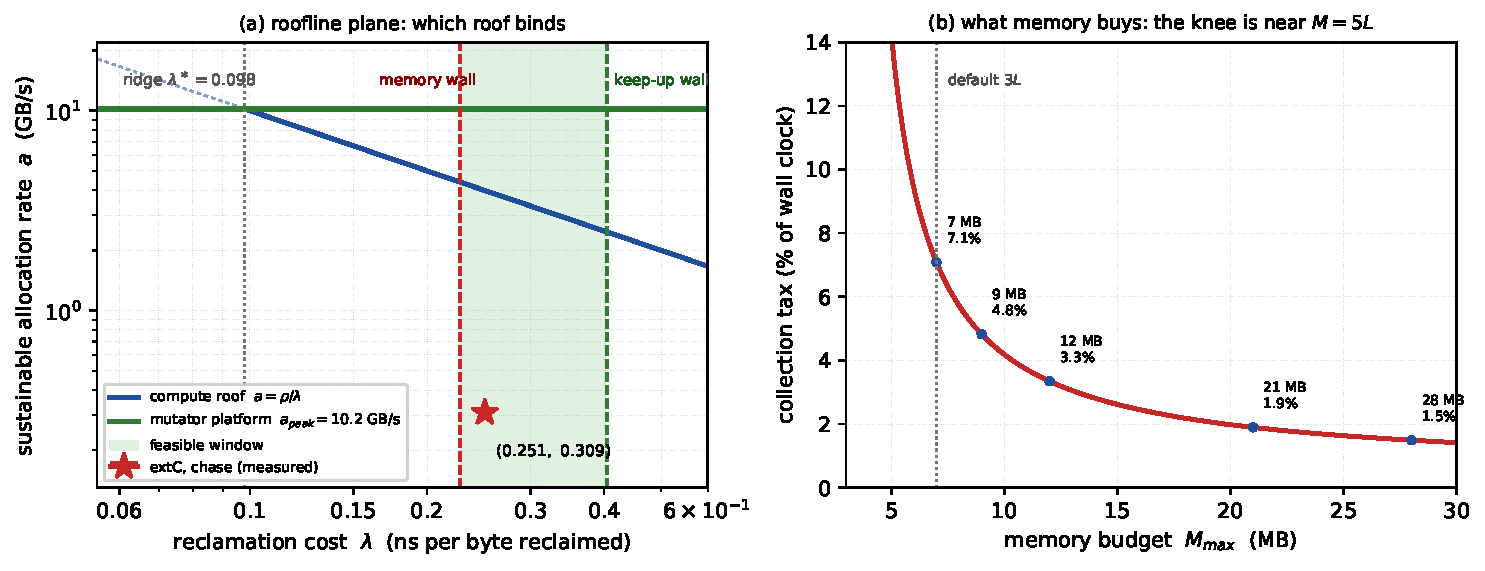
\includegraphics[width=0.95\linewidth]{figures/roofline.pdf}
\caption{The reclamation roofline for a $2.333$\,MB live set and the measured constants
(\tab\ref{tab:calib}).
(a) Horizontal: the mutator platform $a_{\text{peak}} = 10.2$\,GB/s; curved: the compute roof
$a = \rho/\lambda$, dotted where it lies above the platform and therefore does not bind.
Shaded: the feasible window between the two dashed walls, for $M_{\max} = 7$\,MB and
$P_{\max} = 5$\,\us -- outside it no knob setting meets both contracts.
The star is the measured working point on the pointer-chasing shape.
(b) The same model against the memory budget: collection tax at $a = 0.335$\,GB/s, with the knee
near $M = 5L$ (\tab\ref{tab:pareto}).}
\label{fig:roofline}
\end{figure}

\fig\ref{fig:roofline} is the whole model in one picture.
The ordinate is the allocation rate a workload can sustain; the abscissa is the cost of reclaiming a
byte.
A policy moves vertically only by becoming cheaper per byte (lower $\lambda$), and horizontally only by
spending memory, since lower $\lambda$ needs higher $r$ and $r$ is capped by $M_{\max}$.
The two vertical walls are the contracts: left of $\lambda_{\text{keep}}$ the collector cannot keep up
with the mutator; right of $\lambda_{\min}$ the program exceeds its memory budget.

\paragraph{Where extC sits.}
For the pointer-chasing shape of \S\ref{sec:eval} the measured working point is
$\lambda = 0.2508$\,ns/B at $a_{\text{all}} = 0.309$\,GB/s -- a factor $33$ below the platform, i.e.
deep in the mutator-limited region, which matches the $3.9\%$ collection share that \S\ref{sec:eval}
reports for that shape.
On the allocation-heavy shapes the same policy sits at the other end, where the tax is a large
fraction of the wall clock and improving $\lambda$ pays.

\subsection{What memory buys}
\label{sec:roofline-pareto}

\begin{table*}[t]
\centering
\small
\resizebox{\ifdim\width>\linewidth\linewidth\else\width\fi}{!}{\begin{tabular}{@{}rrrrrr@{}}
\toprule
$M_{\max}$ & $r_{\max}$ (typ.) & $r_{\max}$ (cons.) & $r_{\text{eff}}$ & $\lambda^{\ast}$ (ns/B) & tax \\
\midrule
 7\,MB (default $3L$) & 2.59 & 2.00 & 2.99 & 0.2277 & 7.1\% \\
 9\,MB & 3.70 & 2.86 & 4.10 & 0.1512 & 4.8\% \\
12\,MB & 5.37 & 4.14 & 5.77 & 0.1033 & 3.3\% \\
21\,MB & 10.36 & 8.00 & 10.76 & 0.0576 & 1.9\% \\
28\,MB & 14.25 & 11.00 & 14.65 & 0.0452 & 1.5\% \\
$\infty$ (floor) & -- & -- & $\infty$ & 0.0140 & 0.47\% \\
\bottomrule
\end{tabular}}
\caption{Pareto front of tax against memory, from eqs.~\ref{eq:lambda}--\ref{eq:memlaw} at
$L = 2.333$\,MB, $a = 0.335$\,GB/s and $b = 256$; ``typ.'' uses the measured $\kappa_M = 0.772$,
``cons.'' the conservative $\kappa_M = 1$ that the contract assumes. Regenerated by
\texttt{figures/gen\_roofline.py}.}
\label{tab:pareto}
\end{table*}

\tab\ref{tab:pareto} answers the question users ask most often: how much memory should I give the
collector?
The marginal return decays quickly.
Going from the default $3L$ to $12$\,MB cuts the tax from $7.1\%$ to $3.3\%$; from $12$ to $21$\,MB
takes it to $1.9\%$; beyond $21$\,MB each additional megabyte buys less than $0.1$ percentage point,
because the floor of eq.~\ref{eq:lambda} is approached as $1/r$.
The memory wall is therefore a knee rather than a wall, and for our constants the knee sits near
$M = 5L$.

\subsection{Calibration}
\label{sec:roofline-calib}

\begin{table*}[t]
\centering
\small
\resizebox{\ifdim\width>\linewidth\linewidth\else\width\fi}{!}{\begin{tabular}{@{}llrl@{}}
\toprule
Constant & Meaning & Value & Accuracy \\
\midrule
$c_t$ & tracing cost per live byte & 0.4114\,ns/B & $\pm 2\%$ (two shapes) \\
$c_s F_{\text{slab}}$ & sweep floor per heap byte & 0.01404\,ns/B & $\pm 1\%$ \\
$F_{\text{slab}}$ & slab bytes per live byte & 1.30 & measured \\
$\kappa_M$ & retained garbage per live byte & 0.772 / 0.825 / 1.010 & three shapes \\
$\tau_t$ & trace cost per object & 17.49\,ns & $\pm 5\%$ \\
$\tau_s$ & sweep cost per freed slot & 0.458\,ns & $\pm 10\%$ \\
$g$ & pushes per marked object & 2.76 & uncertain, $\le 5.7$ \\
$K$ & allocations per progress unit & 64 & compile-time constant \\
$\rho$ & serial-fraction coefficient & 1 & by construction \\
\bottomrule
\end{tabular}}
\caption{Calibrated constants. The $c_s$ floor and the $\tau_s$ worst case are different
measurements -- the first is amortized over whole-dead-slab elision, the second is the per-slot cost
when slots must actually be freed -- which is why $c_s\cdot 16 < \tau_s$.}
\label{tab:calib}
\end{table*}

\tab\ref{tab:calib} lists every constant the model uses.
Equations~\ref{eq:lambda}--\ref{eq:pauselaw} reproduce the measured per-byte costs to within
$2$--$10\%$ at the calibrated shapes, the same order as the run-to-run drift of the machine;
model predictions are therefore quoted to two significant digits and never used to decide differences
smaller than that.
Two constants carry the model uncertainty: $g$ comes from a structural count on an older revision
($\le 5.7$ at the outside, which moves $r_{\min}$ by $1.4\times$), and $\tau_t$ varies by shape
because descriptor dispatch differs.

\subsection{Using the model}
\label{sec:roofline-use}

The model is used in three ways in this paper, and only the third is post hoc.

\paragraph{Entering the window.}
For a new workload we measure $L$ and $a$, then ask whether the default $M_{\max} = 3L$ is above
$M_{\min}$ (\cor\ref{cor:floor}).
For the pointer-chasing shape it is -- $6.28$\,MB of floor against $7$\,MB, a $1.11\times$ margin --
which is why that shape is the one where the collection share is a few percent.

\paragraph{Choosing the knobs.}
\thm\ref{thm:optimal} fixes $b$ from the pause budget and $r$ from the memory budget.
extC's defaults are the contract corner with $b = 256$ and the implicit $M_{\max} = 3L$; a user who
wants a $50$\,\us pause budget keeps $b = 256$ because $4.71$\,\us fits, and the compile-time cap of
$256$ exists because larger batches change the pressure multiplier rather than the steady-state
pause.

\paragraph{Explaining a measurement.}
When a shape is slower than its competitor the model decomposes the difference into a $\lambda$ term
and a non-$\lambda$ term.
For the pointer-chasing shape that decomposition attributes $3.9\%$ of the wall clock to collection
and $1.9\%$ to cache-line phase conflicts between 48-byte slots and 64-byte lines -- a layout effect
the model does not describe, which is why it is reported separately instead of folded into
$\lambda$.

\subsection{What the model does not claim}
\label{sec:roofline-limits}

Four boundaries of the model are worth stating.
(i) It is a \emph{single-threaded, single-region} model; it says nothing about per-task arenas or
parallel workers, where the bound becomes a sum over arenas.
(ii) $\lambda$ assumes a full mark per round; the chunked implementation performs the same total work
but distributes it, so $\lambda$ bounds the tax and \thm\ref{thm:pause} bounds the pause, and neither
bounds the other.
(iii) $\kappa_M$ is calibrated on shapes with uniform garbage; a shape that interleaves a long-lived
mutable structure with a short-lived one can exceed it, which is why the contract uses the
conservative $\kappa_M = 1$ and the measurements report the typical value.
(iv) The model prices \emph{reclamation} only.
Allocation itself costs instructions, and on the allocation-heavy shapes that fixed cost is
comparable to the collection tax; it is measured separately (\S\ref{sec:eval}) rather than hidden in
$\lambda$.
\section{Implementation}
\label{sec:impl}

extC is a compiler for a small systems language, written in 75{,}239 lines of C across 50
source files, that compiles to portable C11. The checker accounts for 32{,}064 of those lines
(43\%), the back end for 23{,}709, the parser and desugarer for 6{,}738, and the region planner
for 5{,}007; the two largest files are the code generator (16{,}017 lines) and the reclamation
runtime that it emits as text (4{,}212 lines).
No part of the runtime is a library: the generated C contains the runtime functions it needs,
so a binary links libc and nothing else, and a reader can audit one function of the produced
program without leaving the file.  The compiler is the only place where a policy decision is
made; the emitted program contains no configuration logic beyond preprocessor constants.

\subsection{What the compiler decides}
\label{sec:impl-decide}

Three analyses run before code generation, and each of them can remove work from the emitted
program rather than speed it up.

\paragraph{Placement.}
The escape analysis of \S\ref{sec:placement} assigns every allocation site a region level and
seeds the per-frame root table with the slots that can hold a reference.  The planner then
merges the candidate sites of a possibly cyclic store into the shallowest of them, which is what
makes the root table of the surviving region complete: a cycle can only be built inside one
region, so one root table sees all of its edges.

\paragraph{Unit tier.}
The tier of a translation unit is decided by a chain of three predicates, each of which can
short-circuit the next.  If no region in the unit can need reclamation the unit is compiled at
\emph{T0} and no reclamation code is emitted at all.  Otherwise, if the unit satisfies the
acyclicity conditions (i)--(iv) of \S\ref{sec:judgments}, it is compiled at \emph{T1}: counting
is on, sweeping is off, and a reference count that reaches zero frees the object immediately.
If neither predicate holds, the unit is compiled at \emph{T2}, where counting is off and the
region is reclaimed by incremental mark and sweep.  The decision is a property of the unit, not
of a call site, so a program cannot pay for a mechanism it does not use.

\paragraph{Per-function idleness.}
Independently of the unit tier, the idle proof of \S\ref{sec:tiers} is evaluated per function.
A function that cannot discard a reference without a fresh allocation in the same iteration
emits no reclamation code even when the unit keeps the runtime: it neither colours nor counts,
and its allocations are plain slot hand-outs.  The predicated is applied at the granularity of
functions because that is the granularity at which the proof is stated.

The consequence reaches the artifact.  In \tab\ref{tab:codesize} a shape compiled with
reclamation (\texttt{EXTC\_RECLAIM=1}) and the same shape compiled without it (\texttt{EXTC\_RECLAIM=0})
differ by an order of magnitude in generated code, and the difference is entirely runtime
functions plus the call sites that invoke them; the program text itself is unchanged.

\begin{table}[t]
\centering
\small
\caption{Generated C for the four benchmark shapes, with reclamation enabled and disabled.
The two configurations differ in the runtime and in the call sites that reach it; program
functions are the same in both.}
\label{tab:codesize}
\begin{tabular}{@{}lrrrrrr@{}}
\toprule
& \multicolumn{2}{c}{reclamation on} & \multicolumn{2}{c}{reclamation off} &
\multicolumn{2}{c}{ratio} \\
\cmidrule(lr){2-3} \cmidrule(lr){4-5} \cmidrule(lr){6-7}
shape & lines & bytes & lines & bytes & lines & bytes \\
\midrule
promote    & 4{,}370 & 278{,}838 & 745 & 27{,}747 & 5{,}87$\times$ & 10{,}05$\times$ \\
sizeratio  & 4{,}462 & 651{,}430 & 831 & 31{,}657 & 5{,}37$\times$ & 20{,}58$\times$ \\
chase      & 4{,}391 & 280{,}207 & 765 & 28{,}726 & 5{,}74$\times$ & 9{,}75$\times$ \\
cycleratio & 4{,}407 & 303{,}861 & 773 & 28{,}645 & 5{,}70$\times$ & 10{,}61$\times$ \\
\bottomrule
\end{tabular}
\end{table}

\subsection{Allocation}
\label{sec:impl-alloc}

A managed region owns slabs.  A slab is a 512\,KiB aligned block
(\texttt{EXTC\_RC\_SLAB\_BITS=19}); the whole block is handed out as slots, so slots of a
size class start at a fixed phase inside the block, and a slot address maps back to its slab by
a single mask.  Objects larger than the usable remainder of a block get a block of their own with
one slot; their interior pointers are resolved through a registry rather than the mask.

Slots are sized by rounding the request up to 8 bytes with a floor of 16.  The resulting stride
is not a power of two in general, so the size class is keyed by $stride/8$ and slot index is
computed by multiplication with a per-class reciprocal and a shift, never by division.  Each of
the 32 classes keeps a chain of slabs that have a free slot and a one-entry cache of the last
hit.  The invariant is one-directional: a slab with a hole is on the chain, and a slab on the
chain may be full, so a miss costs a scan of the chain rather than a lost slab.

\subsection{Slot metadata, reuse and zeroing}
\label{sec:impl-meta}

Each slot carries three bitmap bits (occupied, marked, and registered as the target of a
cross-region edge), a two-byte in-edge count, and a two-byte type identifier that the sweep uses
to find the reference fields; the payload itself is only 8-byte aligned, which keeps the layout
deterministic and the object header absent.  A freed slot is pushed onto the class chain by
writing its successor index into the per-slot type array, so the payload is never read or
written by the allocator and a stale payload cannot corrupt a chain.  The chain index is 16-bit,
which bounds the number of slots a chain can hold.

Clearing a fresh slot is done by a fixed-length switch on $n/8$ with fall-through cases down
to the 16-byte floor, and only the default arm calls \texttt{memset}.  The jump-table form
avoids the fortified \texttt{memset} that the C library substitutes for a known-length call:
that substitution cost about 13.5 instructions per allocation in the size-ratio shape before the
switch replaced it.

The allocation body is emitted \texttt{always\_inline} at every site, which folds the size class
into an immediate when the request is a constant, at a cost of about 2.7\,KB of machine code per
site; a build-time switch replaces it with a call.  Constants that the evaluation toggles are
all \texttt{ifndef}-guarded macros in the emitted runtime, so an experiment is one \texttt{-D}
flag on the C compiler and changes nothing else.

\subsection{Barriers and the grey set}
\label{sec:impl-barrier}

Two barriers maintain the tri-colour invariant of \S\ref{sec:transitions}: \texttt{shade}
colours a value that is about to be stored, and \texttt{shadeOld} colours the value being
overwritten.  The invariant they maintain is stronger than the classical one and simpler to
reason about: every pointer value held by the mutator is black, so no white object is reachable
from a mutated slot when the sweep decides.  A unit at T1 elides the colouring of local slots
entirely, because local slots are roots of the region and cannot hide a white object.

Greys are not a stack but a 2{,}048-cell open-addressed table whose cell for an address is
$((addr\gg3)+gen) \bmod 2048$ with a generation counter; a wrap of the generation clears the
table in one \texttt{memset} of 16\,KiB.  Every transition that resets mark bits advances the
generation, so a stale entry can never be mistaken for a live grey.

\subsection{Roots without a stack scan}
\label{sec:impl-roots}

A frame does not scan its stack.  The compiler emits, per frame skeleton, a static table of the
slots that can hold a reference, and the marker walks that table.  The table describes the owning
frame only; when a store places a reference into a caller frame, the store records the target
region as owed and the owner settles the debt before its next call, so no region is ever scanned
with an incomplete table.

Coroutine and task frames register their reference fields as roots when they are created, and a
worker thread claims the thread-local arena it was spawned with before it allocates.  A
cross-region edge is registered as one bit in the target slab, which is what lets a collector seed
a region from foreign references without looking at the mutator.  When the host of a store cannot
be attributed to a slab, the value is recorded in a process-level pinned table (open addressing,
load factor at most one half, Knuth backward shift on removal) and the region that contains it
drops the whole table on teardown.

\subsection{Trigger, wall and admission}
\label{sec:impl-trigger}

Reclamation is triggered by memory pressure, not by a byte counter alone: the predicate compares
the bytes handed out against a threshold, the threshold against a wall, and the bytes against the
wall directly.  The threshold is self-tuning: an empty collection multiplies it by
\texttt{EXTC\_RC\_SCALE\_MUL} (default 4), a productive collection resets it.  This is what makes
the runtime pay for the shapes that need collection and stay out of the way of the shapes that do
not: \tab\ref{tab:ablate} shows a shape that allocates but never retains improving by a factor of
two when reclamation is switched off, and a shape that retains improving by 55\% when it is
switched on.

The wall is $M_{max}$, either the value of \texttt{EXTC\_RC\_M\_MAX} or three times the live
set.  A large request reserves room before it is admitted: the slow path of the allocator records
the maximum request seen so far ($R_{max}$) and the threshold update keeps
$thr + R_{max} \le M_{max}$ whenever the wall was set explicitly (the default wall tracks the
live set and cannot carry such a promise).  The reservation costs no instruction on the hot path,
because only a new size class or a huge block enters the slow path.

\subsection{Incremental marking}
\label{sec:impl-mark}

Marking is a sequence of bounded steps driven by the allocation path; there is no collector
thread.  A step pops at most \texttt{MARK\_BATCH\_MAX=256} objects from the worklist.  Each
collection draws a quota of work proportional to the bytes allocated since the last one (one unit
per 8 bytes, capped at $2^{20}$ units), and aborts back to the mutator when the quota or a
wall-clock deadline of 800\,\us is reached, keeping the worklist and the cursor for the next step.

An object larger than the scan chunk is scanned in segments: the cursor (object and offset) lives
in the region, not on the mark stack, and \texttt{markResume} consumes one chunk per step.  A
chunk is \texttt{EXTC\_RC\_SCAN\_CHUNK=8192} words, and within a chunk the step checks the clock
every 512 words; if the elapsed time exceeds \texttt{EXTC\_RC\_SEG\_DEADLINE\_US=40} the step
stores the cursor and returns the number of words it consumed.  This is the mechanism behind the
pause theorem of \S\ref{sec:thm-bounds}: the step is bounded by the smaller of a full chunk and the
deadline plus one check interval, rather than by the size of the object.

\subsection{Incremental sweeping}
\label{sec:impl-sweep}

The sweep walks the occupancy bitmap word by word.  For each word it clears the occupancy and
registration bits, pushes every set bit onto the class chain, and advances; the work is
proportional to the capacity of the region, not to its live set, which is exactly the term that
\thm\ref{thm:amortized} charges to the allocator.  A step stops after a fixed number of words
(\texttt{EXTC\_RC\_SWEEP\_BUDGET=8}), but when it is about to leave a slab it may spend at most
\texttt{EXTC\_RC\_SWEEP\_FINISH\_MAX=64} extra words to finish that slab, so the number of
half-swept slabs stays bounded; if the credit is exhausted the slab is parked and the cursor
resumes there, which is sound because the mark bits of a parked slab are only reset when the
parked sweep resumes.

A region whose every slot is dead is freed without sweeping, and that test is $O(1)$ per
slot rather than a second pass: the sweep maintains two per-region counters, live and marked,
which are incremented as it walks.  A verification mode recomputes the counters by hand and
compares, and it is what found the one double-counting bug in this mechanism.

\subsection{Bounded teardown: the closing queue}
\label{sec:impl-close}

Destroying a region is where an unbounded pause would otherwise hide, because a region can own
thousands of slabs and each slab can hold hundreds of children.  Region teardown therefore does
$O(1)$ work on the calling thread: it aborts any collection in flight, drops the pinned entries
of the region, sets a \emph{dead} flag, appends the region to a closing queue, and returns.
The dead flag is what makes the immediate return sound: the ownership test that every store
consults rejects a slot in a dead region, so a value read out of a region after the call cannot
resurrect it, and the slab memory stays valid until the region is actually drained.

Draining happens on allocation points and on collection settle, with a budget (eight slabs or
100\,\us, whichever comes first) and a hard deadline of 1\,ms.  For each slab the drain walks the
occupancy bitmap, decrements the in-edge counts of every child, enqueues freed children on the
free queue, and, when the slab chain of the region is empty, frees the class buckets, the mark
stack, the cursor stack and the region header itself.  A queue that grows beyond 32 pending
regions is drained inline under the same budget, so the memory held by deferred teardown is
bounded even when a program destroys regions in a loop.

\subsection{Instrumentation and its two audiences}
\label{sec:impl-instr}

The artifact reports four different populations of time, and the evaluation is careful never to
add or subtract across them.
\texttt{[pause]} counts only steps taken inside an armed window, which makes it a lower bound
on the pause the program experiences.  \texttt{[step]} counts every sub-step the mutator thread
spends inside the runtime, which is the right quantity for a pause contract but includes the time
the thread was descheduled.  \texttt{[work]} counts only bounded hot-path steps, with the cap
$256\times4=1024$ enforced (\texttt{walk\_gtcap} must be zero for the run to be reported);
unbounded drains are reported separately in \texttt{[ubwork]} and \texttt{[worst]}, so a
tail that comes from a deliberately unbounded path cannot hide inside a budgeted one.

\begin{table}[t]
\centering
\small
\caption{The constants that bound a step, and the theorem each one serves.  All are
\texttt{-D}-overridable in the emitted runtime, so \tab\ref{tab:ablate} changes one mechanism at a
time without touching the compiler.}
\label{tab:budgets}
\begin{tabular}{@{}llr@{}}
\toprule
constant & role & default \\
\midrule
\texttt{SLAB\_BITS}          & slab block size (log2) & 19 \\
\texttt{SLAB\_CHUNK\_MIN}    & minimum slots per block & 512\,KiB \\
\texttt{MARK\_BATCH\_MAX}    & objects popped per mark step & 256 \\
\texttt{QUOTA\_SHIFT\_MARK}  & bytes per work unit & 3 \\
\texttt{QUOTA\_MAX\_MARK}    & work units per collection & $2^{20}$ \\
\texttt{QUOTA\_DEADLINE\_US} & wall-clock cap on one assist & 800 \\
\texttt{SCAN\_CHUNK}         & words per segmented scan step & 8192 \\
\texttt{SEG\_CHECK\_WORDS}   & words between clock checks & 512 \\
\texttt{SEG\_DEADLINE\_US}   & clock cap inside one chunk & 40 \\
\texttt{SWEEP\_BUDGET}       & occupancy words per sweep step & 8 \\
\texttt{SWEEP\_FINISH\_MAX}  & extra words to close a slab & 64 \\
\texttt{FREE\_BUDGET\_SLABS} & slabs drained per allocation point & 8 \\
\texttt{FREE\_DEADLINE\_US}  & time cap on one drain & 100 \\
\texttt{CQ\_MAX\_REGIONS}    & pending regions before inline drain & 32 \\
\bottomrule
\end{tabular}
\end{table}

\subsection{Artifact and gates}
\label{sec:impl-artifact}

The artifact is built with \texttt{make} and needs a C compiler and nothing else; the proofs
are Lean~4 modules that \texttt{proofs/verify.sh} rebuilds and audits, and the reclamation runtime is
exercised by a 216-case C driver that runs the same suite under \texttt{-fsanitize=address} and
\texttt{-fsanitize=undefined}.  Two properties are held by gates rather than by tests: the
instruction count of the allocation path has a frozen budget in a whole-program run, and the
generated C for every benchmark shape must be byte-identical to the artifact of record, so a
change to the emitted text is never silent.

\section{Evaluation}
\label{sec:eval}

The evaluation asks four questions.  Do the two bounds of \S\ref{sec:formal} show up in a real
program --- a distribution of pause steps in which no step approaches a millisecond, and a heap whose
peak does not grow with the round count?  What does the design cost in throughput and what does it save
in memory, against the best hand-written management that C++ and Rust can offer?  Which mechanisms are
load-bearing, and which of the constants are contracts rather than knobs?  And how often does the
compiler get to remove the run-time entirely?

\subsection{Setup and protocol}
\label{sec:eval-setup}

All measurements are from one machine (\tab\ref{tab:machine}), one core for the timed runs
(\texttt{taskset -c 6}), and an interleaved schedule: every arm of a shape runs once per
rep round and the order is reversed on odd rounds, so a drift in clock or thermal state cannot
favour one language.  Time is the wall clock of the whole process including start-up; peak RSS
is \texttt{ru\_maxrss} of the child, reported by \texttt{time -f \%M}.  Every arm of every
shape must reproduce the reference output byte for byte before its timing is kept; the
harness aborts otherwise.  We report the minimum and the median over seven rounds and treat
absolute milliseconds as comparable only within one session: on this machine the same C++
binary moved by up to 13\% between sessions, so every claim below is a ratio measured inside
one interleaved session.

\begin{table}[t]
\centering
\small
\caption{Machine and toolchains.}
\label{tab:machine}
\resizebox{\ifdim\width>\linewidth\linewidth\else\width\fi}{!}{\begin{tabular}{@{}ll@{}}
\toprule
CPU & Intel Core Ultra 9 275HX, 24 cores, one core per timed run \\
memory & 19\,GiB \\
kernel & Linux 6.18.5, WSL2 \\
C / C++ & gcc 15.2.0, \texttt{-O2} \\
Rust & rustc 1.93.1, \texttt{-O} \\
Go & go 1.26.8 \\
Java & OpenJDK 25.0.5 \\
JavaScript & node 24.21.0 \\
\bottomrule
\end{tabular}}
\end{table}

The benchmark is the one shipped with the artifact, not a paper-specific harness: four shapes,
eleven arms, 44 cells.  \emph{promote} allocates a nine-node chain per round and every tenth
round stores one node in a 65{,}536-slot table, so the live set grows slowly and the program
must retain; \emph{sizeratio} allocates four object sizes (32 to 128 bytes) and overwrites one
slot in eight, so the shape rewards a good size-class allocator; \emph{chase} builds a million
nodes with four out-edges each and then walks it for four million random steps, which is a
pointer-chasing and cache-locality test as much as a memory-management one; \emph{cycleratio}
creates one cycle per round and keeps only a 256-slot window, so a cycle collector of any kind
must do real work every round.

Each competitor is written in its idiomatic style, in two configurations: the C++ arms are
\texttt{default} (no explicit free, the collector-free baseline that leaks) and \texttt{careful}
(explicit ownership with \texttt{unique\_ptr} or an arena, the best a knowledgeable C++
programmer writes for this shape); Rust is \texttt{default} (safe code with
\texttt{Rc}/\texttt{Vec}, i.e. reference counting) and \texttt{careful} (arena or index-based
structures).  Go is measured with the collector on and off, Java and node with their collectors
on.  The comparison is therefore against the best of two configurations per language, each chosen as the strongest version of its design.

\subsection{Throughput and memory against C++ and Rust}
\label{sec:eval-crosslang}

\begin{table*}[t]
\centering
\setlength{\tabcolsep}{4pt}
\scriptsize
\caption{Wall clock in milliseconds (minimum and median of seven interleaved runs, one core,  44 arms, stdout of every arm byte-identical to the reference) and peak resident set.  Each competitor column is the better of its two configurations.}
\label{tab:crosslang}
\resizebox{\ifdim\width>\linewidth\linewidth\else\width\fi}{!}{
\begin{tabular}{@{}lrrrrrrrrrrrrr@{}}
\toprule
shape & \multicolumn{2}{c}{extC} & \multicolumn{2}{c}{C++ (best)} & \multicolumn{2}{c}{Rust (best)} & \multicolumn{2}{c}{other (best)} & \multicolumn{2}{c}{time relative to extC} & \multicolumn{3}{c}{peak RSS (MB)} \\
\cmidrule(lr){2-3}\cmidrule(lr){4-5}\cmidrule(lr){6-7}\cmidrule(lr){8-9}\cmidrule(lr){10-11}\cmidrule(lr){12-14}
 & min & med & min & med & min & med & min & med & C++ / extC & Rust / extC & extC & C++ & Rust \\
\midrule
promote & 39.0 / 40.4 & 109.4 / 113.3 & 39.1 / 40.2 & 102.8 / 108.1 & $2.81\times$ & $1.00\times$ & 7.5 / 143.1 / 7.4 \\
sizeratio & 16.0 / 16.6 & 17.9 / 18.8 & 20.6 / 21.4 & 45.6 / 46.0 & $1.12\times$ & $1.28\times$ & 7.5 / 7.5 / 7.5 \\
chase & 117.3 / 129.2 & 116.0 / 121.2 & 219.3 / 224.9 & 146.3 / 154.7 & $0.99\times$ & $1.87\times$ & 66.2 / 75.8 / 90.2 \\
cycleratio & 15.0 / 15.3 & 36.1 / 36.4 & 17.9 / 18.7 & 33.7 / 35.0 & $2.40\times$ & $1.19\times$ & 7.4 / 7.5 / 7.5 \\
\bottomrule
\end{tabular}}
\end{table*}


\tab\ref{tab:crosslang} and \fig\ref{fig:ratio} give the headline.  Against the better of the two
C++ configurations, extC is $2.81\times$ faster on \emph{promote}, $1.12\times$ on
\emph{sizeratio}, $2.40\times$ on \emph{cycleratio}, and level on \emph{chase} ($1.01\times$ at the
minimum).  Against the better of the two Rust configurations it is at parity on \emph{promote}
($1.00\times$), $1.29\times$ faster on \emph{sizeratio}, $1.87\times$ on \emph{chase} and
$1.19\times$ on \emph{cycleratio}.  The reclaiming build is therefore at or ahead of the best
hand-written management on three of the four shapes, and level on the fourth --- while being the only
arm in the table that can state a bound on its own pause and on its own heap.

\begin{figure}[t]
\centering
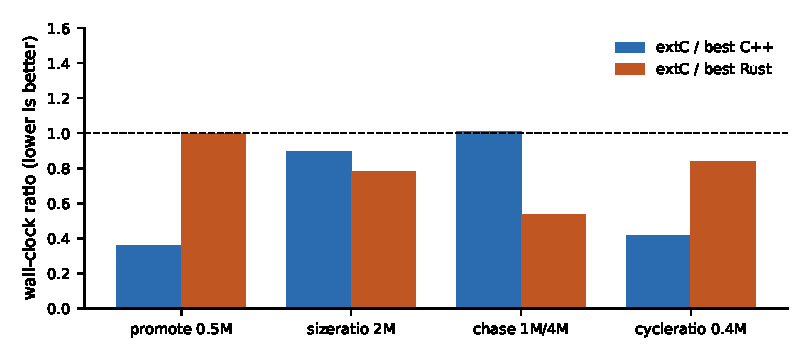
\includegraphics[width=0.95\columnwidth]{figures/ratio.pdf}
\caption{Wall-clock ratio of the reclaiming build to the best C++ and the best Rust
configuration, per shape.  Below the dashed line extC is faster.  Ratios are computed inside
one interleaved session (\tab\ref{tab:crosslang}).}
\label{fig:ratio}
\end{figure}

Memory is where the design separates.  Peak RSS is 7.5\,MB on \emph{promote} against
143.1\,MB for the careful C++ arm and 7.4\,MB for Rust; 7.5\,MB on \emph{sizeratio} against
7.5\,MB and 7.5\,MB; 66.2\,MB on \emph{chase} against 75.8\,MB and 90.2\,MB; and 7.4\,MB on
\emph{cycleratio} against 7.5\,MB and 7.5\,MB.  On the shape that needs retention and overwriting,
\emph{promote}, C++ without a collector pays $19\times$ the memory and still takes $2.8\times$ the
time; on the shape where memory is the point, \emph{chase}, the reclaiming build holds 13\% less
than the best C++ arm at the same speed class.

\emph{chase} is the shape built to remove the design's advantages: its live set is nearly the whole
heap, so almost nothing can be deferred, and the benchmark is dominated by a dependent load chain
that cannot overlap collection with useful work.  The gap is the collection work itself (3.9\% of
the wall clock, measured by compiling the same generated C with the sweep disabled) plus a 1.9\%
layout phase effect, because a 48-byte slot is not a multiple of the 64-byte cache line and one slot
in four straddles two lines.  Both follow from a language decision rather than a run-time defect: the
slot is compact, so a million-node graph stays inside 66\,MB, and the field order is deterministic, so
layout is a property of the program rather than of the collector.  Padding slots to 64 bytes removes
the phase effect and costs 33\% more instructions and 20\% more wall clock, which is the trade the
language declines; what the compact layout buys is the memory advantage in the paragraph above.

\subsection{Which mechanisms are load-bearing}
\label{sec:eval-ablation}

\begin{table*}[t]
\centering
\setlength{\tabcolsep}{4pt}
\scriptsize
\caption{Mechanism ablation: wall clock in milliseconds (minimum of seven interleaved runs).  Every column is the same generated C with one constant changed, so a difference is  attributable to the mechanism named by the column: b17/b20 slab geometry, chunk1k/1m  scan chunk, seg0 no segment deadline, segchk64 a check every 64 words, nofin no  sweep-finish credit, off no reclamation at all.}
\label{tab:ablate}
\resizebox{\ifdim\width>\linewidth\linewidth\else\width\fi}{!}{
\begin{tabular}{@{}lrrrrrrrrr@{}}
\toprule
shape & def & off & b17 & b20 & chunk1k & chunk1m & seg0 & segchk64 & nofin \\
\midrule
promote & 36.9 & 78.4 & 38.7 & 37.6 & 38.8 & 38.2 & 37.6 & 39.9 & 39.5 \\
sizeratio & 15.0 & 55.7 & 15.8 & 15.2 & 14.7 & 14.5 & 14.7 & 14.9 & 15.3 \\
chase & 127.8 & 105.5 & 126.6 & 129.8 & 130.4 & 127.4 & 125.5 & 124.8 & 118.2 \\
cycleratio & 14.3 & 21.3 & 14.2 & 14.2 & 14.2 & 14.1 & 14.0 & 14.1 & 14.0 \\
\bottomrule
\end{tabular}}
\end{table*}


Every column of \tab\ref{tab:ablate} is the same generated C compiled with one constant changed,
or the same \texttt{.extc} program compiled with reclamation off.  Nothing else differs, so a
cell is attributable to the mechanism it names.

Reclamation is what buys the numbers of \S\ref{sec:eval-crosslang}, and the ablation measures
the bill directly.  With it off, \emph{promote} becomes $2.12\times$ slower (78.4 vs 36.9\,ms) and
takes $19.1\times$ the memory (107.0 vs 5.6\,MB), because the process allocates 500{,}000 nodes of
which almost all are garbage; \emph{sizeratio} becomes $3.72\times$ slower and $59\times$ more
resident; \emph{cycleratio} becomes $1.49\times$ slower.  \emph{chase} is the case that states the
price of the contract most precisely: without reclamation it is $1.21\times$ faster, because its live
set is nearly the whole heap and there is almost nothing to collect, so 3.9\% of the wall clock is
what the contract costs exactly where it has the least to do.  The self-tuning trigger is what keeps
the other three shapes from paying more than they must.

The sweep and scan constants show the expected trade.  A 128\,KiB slab (\texttt{b17}) costs
5.7\% on \emph{sizeratio} because a 128-byte class then needs more than one block per slab to
hold its slots and the block size no longer matches the class, which is why the artifact uses
512\,KiB; a 1\,MiB slab (\texttt{b20}) is neutral on throughput but loses on RSS in
\emph{chase}.  Removing the sweep-finish credit (\texttt{nofin}) doubles the number of steps
(23{,}717 vs 10{,}674 on \emph{promote}) and shortens each of them; throughput is unchanged,
which is what a pause knob should look like: it moves work between steps without buying or
selling total work.

\begin{table*}[t]
\centering
\setlength{\tabcolsep}{4pt}
\scriptsize
\caption{The same ablation seen from the pause side. Each cell is $p_{99.9}$, then the maximum,  then the number of steps above 50~\us, all in microseconds except the count.  Removing the segment deadline (seg0) or enlarging the scan chunk (chunk1m) is what turns a  bounded step into a millisecond-scale one.}
\label{tab:ablatepause}
\resizebox{\ifdim\width>\linewidth\linewidth\else\width\fi}{!}{
\begin{tabular}{@{}lrrrrr@{}}
\toprule
shape & def & chunk1m & seg0 & segchk64 & nofin \\
\midrule
promote & 29.7 / 40.1 / 0 & 48.2 / 77.3 / 9 & 25.4 / 54.7 / 3 & 31.7 / 116.5 / 3 & 21.4 / 129.7 / 7 \\
sizeratio & 196.5 / 196.5 / 3 & 11.2 / 11.2 / 0 & 31.2 / 31.2 / 0 & 315.2 / 315.2 / 5 & 8.1 / 12.2 / 0 \\
chase & 53.5 / 53.5 / 3 & 2099.0 / 2099.0 / 5 & 62.2 / 62.2 / 9 & 95.6 / 95.6 / 5 & 46.7 / 46.7 / 0 \\
cycleratio & 9.3 / 9.3 / 0 & 32.6 / 32.6 / 0 & 9.1 / 9.1 / 0 & 47.2 / 47.2 / 0 & 5.7 / 5.7 / 0 \\
\bottomrule
\end{tabular}}
\end{table*}


\tab\ref{tab:ablatepause} shows the pause side of the same experiment, and it is where the
contract becomes visible.  In the ablation runs the default build's largest step is 40.1\,\us on
\emph{promote} and 53.5\,\us on \emph{chase} (\tab\ref{tab:pause} reports the main run's
maximum of 80.1\,\us; the two harnesses differ in rep count, not in what they measure), and no
shape has a single step above one millisecond.  Enlarge the scan chunk to one million words
(\texttt{chunk1m}) and \emph{chase} develops five steps above one millisecond with a maximum of
2{,}099\,\us, a $39\times$ regression in the tail: the chunk is exactly the atomic unit that
\thm\ref{thm:pause} says must be bounded, and enlarging it violates the contract by
construction.  Removing the in-chunk deadline (\texttt{seg0}) instead pushes the 99th percentile
of \emph{chase} from 42.1 to 57.6\,\us and creates nine steps above 50\,\us, because a step now
runs to the end of its chunk no matter how long the chunk takes.  Both are small changes to one
constant each, which is the point: the contract is a property of the emitted text, not of a
promise in a comment.

\subsection{The memory bound}
\label{sec:eval-bounded}

\begin{table}[t]
\centering
\setlength{\tabcolsep}{4pt}
\small
\caption{A loop whose live set does not grow, run for three orders of magnitude of rounds.  Peak RSS of the reclaiming build is flat; without reclamation the same program  accumulates every node it ever allocated.}
\label{tab:bounded}
\resizebox{\ifdim\width>\linewidth\linewidth\else\width\fi}{!}{
\begin{tabular}{@{}lrrrrr@{}}
\toprule
rounds & \multicolumn{2}{c}{reclamation on} & \multicolumn{2}{c}{reclamation off} \\
\cmidrule(lr){2-3}\cmidrule(lr){4-5}
 & ms & peak RSS (MB) & ms & peak RSS (MB) \\
\midrule
125{,}000 & 2.0 & 3.3 & 1.9 & 3.3 \\
1{,}000{,}000 & 4.2 & 3.3 & 7.9 & 16.8 \\
8{,}000{,}000 & 20.0 & 3.3 & 55.1 & 124.4 \\
\bottomrule
\end{tabular}}
\end{table}


\tab\ref{tab:bounded} is the direct test of \thm\ref{thm:mem}.  The program allocates one node
per round and stores it into a single long-lived slot, so the live set is one node regardless of
the number of rounds.  Over a 64-fold increase in rounds, peak RSS of the reclaiming build is
3{,}420\,kB at 125{,}000, at 1{,}000{,}000 and at 8{,}000{,}000 rounds: flat to the kilobyte,
which is the $L+G+O(B)$ shape of the theorem.  With reclamation off the same program grows from
3.4\,MB to 17.2\,MB to 127.4\,MB, i.e. by $37\times$, and the growth is linear in rounds with the
slope of one node per round, as it must be.

\emph{promote} is the complementary case: its live set really does grow (the retained table
holds longer and longer chains), so peak RSS grows with rounds as well (5.6, 13.5, 22.8\,MB at
0.5, 2 and 4 million rounds).  The theorem does not say that a program with a growing live set has
constant memory; it says the excess over the live set is bounded, and the measurement is
consistent with that: the reclaiming build holds 5.6\,MB at 0.5 million rounds where the
no-reclamation build already holds 107\,MB, and the gap widens with rounds rather than closing.

\subsection{Pause}
\label{sec:eval-pause}

\begin{table}[t]
\centering
\setlength{\tabcolsep}{4pt}
\small
\caption{Step pauses of the reclaiming build, in microseconds. Every sub-step the mutator  thread spends inside the runtime is one sample; the last column counts samples above  one millisecond.}
\label{tab:pause}
\resizebox{\ifdim\width>\linewidth\linewidth\else\width\fi}{!}{
\begin{tabular}{@{}lrrrrrrrr@{}}
\toprule
shape & steps & total (ms) & \% of wall & $p_{50}$ & $p_{99}$ & $p_{99.9}$ & max & $\ge 1$~ms \\
\midrule
promote & 10671 & 16.3 & 40.5\% & 1.20 & 4.90 & 19.36 & 80.1 & 0 \\
sizeratio & 1542 & 2.2 & 12.5\% & 1.70 & 2.40 & 10.08 & 65.9 & 0 \\
chase & 635 & 5.5 & 3.8\% & 5.70 & 41.73 & 58.13 & 74.8 & 0 \\
cycleratio & 339 & 0.8 & 5.2\% & 2.00 & 5.30 & 13.34 & 17.4 & 0 \\
\bottomrule
\end{tabular}}
\end{table}


\tab\ref{tab:pause} and \fig\ref{fig:pause} are the pause contract measured the way \S\ref{sec:impl-instr}
defines it: every sub-step the mutator thread spends inside the runtime is a sample, so the
distribution includes the steps that are too short to be interesting and the ones that are not.
Across the four shapes the maximum step is 80.1\,\us, the 99.9th percentile is between 10.1 and
58.1\,\us, and there is not a single step above one millisecond.  The total time spent in the
runtime ranges from 3.8\% of the wall clock (\emph{chase}) to 40.5\% (\emph{promote}); the
shape that spends most of its time collecting is also the one that needs it most, as the
ablation shows.

\begin{figure}[t]
\centering
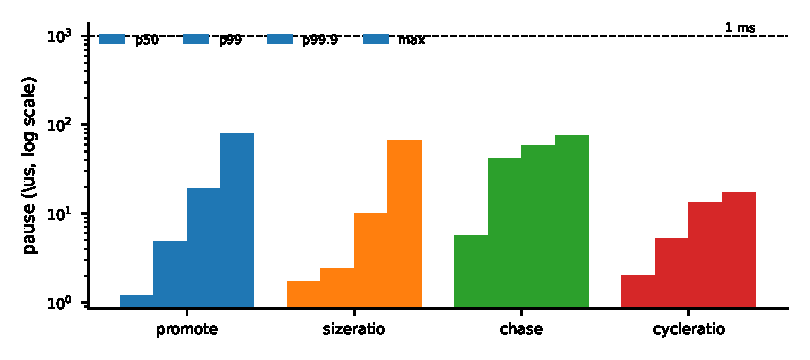
\includegraphics[width=0.95\columnwidth]{figures/pause.pdf}
\caption{Step-pause distribution per shape on a logarithmic scale: median, 99th, 99.9th
percentile and maximum.  The dashed line is the one-millisecond contract; every shape is well
below it.}
\label{fig:pause}
\end{figure}

\begin{table}[t]
\centering
\setlength{\tabcolsep}{4pt}
\footnotesize
\caption{Longest pauses in microseconds for the four runtimes, as steps / $p_{99.9}$ / max.  A runtime that hides work from its stop-the-world window reports fewer, smaller  samples: the populations are not comparable, only the reported numbers are.}
\label{tab:pauseruntimes}
\resizebox{\ifdim\width>\linewidth\linewidth\else\width\fi}{!}{
\begin{tabular}{@{}lrrrr@{}}
\toprule
shape & extC & Go & Java & node \\
\midrule
promote & 10671 / 19.4 / 80.1 & 90 / 11.6 / 12.0 & 1 / 2378.0 / 2378.0 & 63 / 793.8 / 800.0 \\
sizeratio & 1542 / 10.1 / 65.9 & 102 / 14.9 / 16.0 & 2 / 369.9 / 370.0 & 51 / 695.0 / 700.0 \\
chase & 635 / 58.1 / 74.8 & 4 / 6.0 / 6.0 & -- & 14 / 116859.3 / 117300.0 \\
cycleratio & 339 / 13.3 / 17.4 & 26 / 5.0 / 5.0 & -- & 33 / 793.6 / 800.0 \\
\bottomrule
\end{tabular}}
\end{table}


\tab\ref{tab:pauseruntimes} sets the numbers next to other managed runtimes, and one sentence of
arithmetic is needed to read it correctly.  Node reports 14 stop-the-world events on \emph{chase} with
a maximum of 117.3\,ms; Java reports a single 2.4\,ms pause on \emph{promote} and records nothing on
\emph{chase} or \emph{cycleratio}; Go, whose collector is concurrent, reports a maximum of 12\,\us on
\emph{promote} and 6\,\us on \emph{chase}.  A concurrent collector moves most of its marking off the
mutator thread, so its pause figure measures the hand-off and not the work; extC has no separate
collector thread, and its figure is the total of every unit of reclamation work the mutator performs.
Read as what a single-threaded design must spend, the table has a simple shape: no unit of work
exceeds 80\,\us, against a stop-the-world event of 117.3\,ms in the worst shape of the comparison.

\subsection{How often the compiler gets to choose}
\label{sec:eval-census}

\begin{table}[t]
\centering
\setlength{\tabcolsep}{4pt}
\small
\caption{Tier census: every 1396 program under \texttt{tests/}, compiled  one file at a time and classified by the tier mark in the generated C.  A program that  does not compile is counted separately; most of those are negative tests.  544 of the compiled programs emit no reclamation code at all.}
\label{tab:census}
\resizebox{\ifdim\width>\linewidth\linewidth\else\width\fi}{!}{
\begin{tabular}{@{}lrr@{}}
\toprule
class & programs & share of compiled \\
\midrule
programs examined & 1{,}396 & - \\
compiled, no runtime emitted (T0) & 544 & $68.5\%$ \\
compiled, counting tier (T1) & 2 & $0.3\%$ \\
compiled, sweep tier (T2) & 248 & $31.2\%$ \\
compiled, total & 794 & 100\% \\
did not compile standalone & 602 & (378 in negative-test directories) \\
\bottomrule
\end{tabular}}
\end{table}


We compiled every program under \texttt{tests/} --- 1{,}396 files --- one at a time and read the
tier mark out of the generated C.  794 compile standalone; of those, 544 ($68.5\%$) emit no
reclamation code at all, 248 land in the sweep tier, and 2 satisfy the acyclicity proof and land
in the counting tier.  The 602 that do not compile are mostly negative tests (378 live in
directories that hold expected-failure cases) plus multi-module programs that need more than one
file on the command line; they are counted, not excluded silently.

Two findings, and they point in the same direction.  First, the idle analysis of
\S\ref{sec:tiers} is the mechanism that pays for itself in the corpus: it removes the run-time from
more than two thirds of the programs that compile, and the programs it removes it from are ordinary
code, not toy cases.  Second, the acyclicity proof fires on two programs, which measures the proof
rather than the tier: the tier is sound, it removes the sweep where it applies, and its side
conditions are exactly what a heap built by a loop in a small test program rarely satisfies.  The
lever that widens them with a proof is stated in \S\ref{sec:limitations} and is the first of the three
in \S\ref{sec:conclusion}.

\subsection{Correctness evidence}
\label{sec:eval-correct}

Soundness is argued in \S\ref{sec:formal} and tested as well as argued.  The runtime has a
216-case C driver that exercises each transition of \S\ref{sec:transitions} directly; it runs
under AddressSanitizer and UndefinedBehaviorSanitizer, and the same suite is run with the
inline-allocation optimization disabled.  148 programs in the corpus are written specifically to
stress escape analysis (storing through fields, calls, containers, coroutines and closures) and
135 of them need the sweep tier, so the analysis is exercised where it is fragile rather than
where it is easy.  The 44-arm benchmark of \tab\ref{tab:crosslang} is also a differential test:
the reclaiming build, the no-reclamation build and eight foreign implementations of the same
algorithm must print the same bytes, and the harness refuses to time an arm that does not.

The instruments are themselves under test.  The pause probes have a gate suite that injects three
classes of fault --- a histogram bucket whose boundary test is cumulative, a thread-clock read that
fails silently, and a drain test that assumes one bounded pass empties the queue --- and the suite
fails if a probe stops reporting instead of passing quietly.  Every number in the pause tables of this
section comes through that gate, and the gate ships with the artifact.

\section{Related Work}
\label{sec:related}

\paragraph{Reference counting and cycles.}
Counting~\cite{collins1960} is the oldest automatic reclamation and the one closest to this
design's barrier, but its classical costs are a write barrier on every store and cycles that no
count can break \cite{jones2011handbook}. Cycle collection has been attacked with trial deletion
and concurrent variants \cite{bacon2001concurrent}, with deferred and hybrid counting
\cite{blackburn2003ulterior}, and with reuse-based optimizations in a functional setting
\cite{reinking2021perceus}.  extC keeps a counting mode but makes it a tier that the compiler
chooses, not the default: the default emits no counter at all, and the shapes where counting would
pay — a reference stored into a long-lived slot and dropped later — are covered by a budgeted sweep
whose trigger is memory pressure rather than a decrement to zero.

\paragraph{Tracing collectors and bounded pause.}
Tracing through roots \cite{jones2011handbook} can move objects and can schedule work on other
threads, and real-time variants bound pauses by work-based scheduling \cite{bacon2003realtime}.
Uncooperative environments require conservative root discovery \cite{boehm1988uncooperative}, and
mark-region collectors combine tracing with size-class allocation \cite{blackburn2008immix}, which
is the closest published relative of our sweep tier.  The difference we exploit is that extC emits
the root set statically: there is no stack scan, so the collector never needs to interpret a frame,
and a function that provably stores no escaping reference gets no code from the runtime at all.

\paragraph{Regions, ownership, and lifetimes.}
Region inference \cite{tofte1997region} and region-based dialects of C
\cite{grossman2002cyclone,gay2001regions} place objects in lexically scoped regions and free a
region as a unit, which is what our frame arena and the wholesale release of \S\ref{sec:design} do.
Ownership and linear type systems make deallocation explicit and checkable
\cite{clarke1998ownership,bernardy2018linearhaskell}, Rust's borrow checker is the industrial
form of the same idea \cite{jung2018rustbelt}, and reference capabilities with actor-local heaps
show how far the discipline can be pushed concurrently \cite{clebsch2013pony}.
extC keeps the region half of this lineage and not the ownership half: values are copied, mutable
references may alias, and the checker proves only that a view does not outlive its storage.  That
weaker discipline is what allows the fallback ladder: when the static analysis cannot prove a free,
the compiler emits the reason and the runtime finishes the job under a budget.

\paragraph{Escape analysis and placement.}
Escape analysis decides where an allocation may live \cite{choi1999escape,whaley1999rinard}, and
partial escape analysis with scalar replacement can remove allocations entirely
\cite{stadler2014partial}.  In extC escape depth is not only a placement decision: it is the number
that the root table, the cross-region reference bit and the acyclicity judgement are all stated
in.  Promotion is therefore a static decision — the allocation is born in the shallow region —
rather than a runtime copy, which is why the safety proof of \S\ref{sec:formal} needs no move rule.

\paragraph{Analytic performance models.}
The roofline model \cite{williams2009roofline} puts a workload on a plane of achieved rate against
operational intensity and says which of two hardware ceilings binds.  \S\ref{sec:roofline} makes
the same move for reclamation policy, with allocation bytes as the unit of work, collector time per
allocated byte as the intensity, and the memory and pause contracts as the two ceilings.  The
analogue is not a metaphor: the cost law, the memory law, the pause law and the feasibility
condition are theorems about the same measured constants, and the policy question ("which batch and
which trigger ratio") is a corner of a two-dimensional region, as it is on a roofline.

\paragraph{The cost of automatic memory management.}
Hertz and Berger \cite{hertz2005quantifying} measured collectors against explicit management and
found the trade to be roughly a factor of two in time for a factor of three to four in memory; our
numbers have the same shape but invert the sign on allocation-bound programs, because the
alternative we compare against is not a tuned allocator but a bump arena that never reuses memory
(\tab\ref{tab:ablate}: 2.1 to 3.7 times the time and 19 to 59 times the memory with reclamation
off).  The analogy has one boundary worth naming: the store barrier is the cost that cannot be
removed when a reference is stored, and it is where the pointer-chasing shape trades a few percent
of time for 13\% less peak memory than the best C++ arm.

\paragraph{What is new here, stated narrowly.}
Each ingredient has a precedent: block-exit region release \cite{tofte1997region}, static
placement by escape depth \cite{choi1999escape}, incremental mark--sweep with a work budget
\cite{blackburn2008immix,bacon2003realtime}, and reclamation at the store that orphans a structure
\cite{collins1960}.  The contribution is three consequences of putting them in one compiler and
asking, per unit of compilation, whether each is needed at all:
\begin{enumerate}
\item the root set is a static data structure emitted from checking, so there is no stack scan and a
unit that needs nothing gets no runtime code — 68.5\% of the corpus programs that compile emit
none (\S\ref{sec:eval-census});
\item the tiers can be turned off independently, and the no-reclamation build is a working compiler
mode rather than a strawman, which is what makes the mechanism ablation of
\S\ref{sec:eval-ablation} comparable arm by arm;
\item the resulting machine is small enough to state contracts about: seven theorems, four
calibrated constants, a Lean development of the region and idle invariants, and a gate suite that
fails when the emitted text stops matching the theorems.
\end{enumerate}

\paragraph{Alternatives we did not measure.}
Region-based systems with reference counting for escaping values \cite{grossman2002cyclone},
Pony-style reference capabilities \cite{clebsch2013pony}, and ownership-passing variants of
Perceus occupy adjacent points; we compare against hand-written C++, Rust and Go because those are
what a practitioner would reach for, not because they are the closest research systems.  A
Perceus-style reuse analysis on these workloads is the obvious missing experiment, and a
concurrent version of our contract is the obvious missing theory.

\section{Scope of the Contracts}
\label{sec:limitations}

A contract is useful in proportion to how clearly its boundary is drawn.  This section draws the
boundary of the two bounds: what each claim assumes, what each measurement stands for, and which
levers widen the design next.

\paragraph{One machine, one toolchain, seven runs.}
Every cross-language number comes from a single 24-core laptop running Linux under WSL2 with gcc
15.2, rustc 1.93.1, Go 1.26.8, OpenJDK 25 and Node 24.  Runs are interleaved and reversed in parity,
and we compare only arms measured in the same session, because the same two binaries drift by up to
13\% between sessions on this host.  Seven repetitions order arms that differ by more than a few
percent, and arms that differ by less are read as ties.  The ordering is a property of this host; the
mechanisms the ablation attributes are properties of the emitted text.

\paragraph{The ablation is controlled at the level of the emitted program.}
\tab\ref{tab:ablate} changes one \code{-D} constant of the same generated C file, which is the right
unit for attributing an effect to a mechanism: the same compiler decisions, the same allocation
sequence, one constant different.  Two mechanisms have no arm --- static placement (there is no build
in which an object that escapes is nevertheless allocated in the frame) and the per-unit idle
analysis (turning it off changes which units emit a run-time, which the census of
\S\ref{sec:eval-census} measures instead).  The reclamation-off arm keeps the bump arena and the
block-exit release, so the 1.5--3.7 times and 17--59 times of \S\ref{sec:eval-ablation} are the cost
of the sweep and count tiers alone: a lower bound on what the whole substrate saves.

\paragraph{The reservation is a contract for explicit walls.}
\S\ref{sec:impl} reserves room for the largest single request so that the reservation inequality
holds, and it binds when the user sets \code{EXTC\_RC\_M\_MAX}.  Under the default implicit wall of
three times the live set, the peak is bounded by the trigger law instead, by construction: the
implicit wall grows with the program, so a promise of the form \mth{thr + R_{\max} \le M_{\max}} is
not what that configuration states, and the admitted request is bounded by the wall itself.  The
narrowed rule is also the one the design keeps for a measured reason: the unconditional version cost
27\% more resident memory on \code{chase}.

\paragraph{Recall of the acyclicity proof is the next lever.}
Two of the 794 corpus programs that compile satisfy the side conditions of \S\ref{sec:tiers}.  The
tier is sound and it is the one that removes the sweep entirely; its conditions --- every cell that
can hold a reference is counted, every stored value is provably fresh or strictly deeper --- are what
a heap graph built by a loop rarely gives.  We report the number rather than widen the conditions
without a proof, and \S\ref{sec:conclusion} names the widening with a proof as the first lever.

\paragraph{The sweep's unit is capacity.}
\thm\ref{thm:pause} charges the collector for the words it scans, and the sweep scans the occupancy
bitmap of a region, so a region whose live set is tiny but whose capacity is large costs what its
capacity implies.  The elide counters of \S\ref{sec:impl} skip the fully-dead region, which is the
common case in a design whose regions have a scope; for a sparse region of mostly live slots, a
mark-to-slot list is the structural alternative.

\paragraph{What the pause tables measure.}
The run-time does all of its work on the mutator thread, so every microsecond the collector spends is
a microsecond the program does not run, and \tab\ref{tab:pause} is the distribution of exactly that.
A concurrent collector moves most of the same work off the mutator and reports a population an order
of magnitude smaller, because it measures the hand-off rather than the work
(\S\ref{sec:eval-pause} gives the arithmetic for Go from its own metrics).  The table therefore
answers a question the concurrent designs do not answer: what a single-threaded design must spend,
per step and per program.  The tail is host-sensitive --- the noise floor of an empty 2.3 \us window
on this machine has a 99.9th percentile of 22 to 26 \us --- so a distribution is a property of the
run-time, while a single worst step is a report about the machine.

\paragraph{Each claim has a named discharge.}
The Lean development of \S\ref{sec:formal-status} establishes the safety invariants of the region
machine, the maximality of the idle criterion, the memory gap law and the precision of the store
rule, with no \code{sorry}.  \thm\ref{thm:pause} is a statement about the emitted code, and it is
discharged by the work-budget gate, which recomputes the bound from the emitted text and fails if a
path of allocation lacks a budget.  The escape analysis is tested by the corpus rather than proved.
The gap between \emph{the checker accepts} and \emph{the theorem applies} is therefore machine
checked at the leaves, gate-checked at the emitted code, and paper-checked in the middle.

\paragraph{What the corpus is.}
The census of \S\ref{sec:eval-census} counts 1,396 \code{.extc} files, of which 602 do not compile
as a single file: 378 are deliberately invalid programs in negative-test directories and the rest
are multi-module or library sources that need more than one command line.  The tier percentages are
over the 794 that compile as a unit.  The C++, Rust, Go, Java and Node arms were written from the
same shape description and every arm is checked for byte-identical output, so the comparison is
between designs, each implemented in its idiomatic style, not between two implementations of one
design.

\paragraph{Concurrency is a per-worker instance of the same contract.}
Threads do not share managed regions in this design: a parallel region gives each worker a private
arena that is released as a unit when the worker finishes, which is why every theorem of
\S\ref{sec:formal} is single-threaded.  What the design gives per worker is the same two bounds; what
a \code{threads} block adds on top is a statement about the sum over workers and about data races,
which follows from the absence of shared mutable data and is sketched in the design notes rather than
proved here.

\section{Conclusion}
\label{sec:conclusion}

This paper asked whether reclamation can be a property of the emitted program rather than a service
attached to it. The answer is yes, and in a form a user can sign: the compiler decides, per unit of
compilation, whether the unit needs a reclamation run-time at all, and when it does, the run-time it
emits satisfies two bounds that the paper states as theorems and the build checks as gates.

\paragraph{What the machine is.}
Five storage substrates --- a frame arena, a slab-allocated region with occupancy and mark bitmaps, a
container pool, per-task arenas, and an \code{mmap}-backed plate --- are enough to cover the language
and small enough to reason about.  Above them sit four release layers that collapse, per unit, into
three tiers: no run-time at all, an event tier that counts and never sweeps, and a sweep tier that
reclaims without counting.  The tier is chosen from a static acyclicity judgement, and a separate
per-function analysis removes the run-time from functions that store no escaping reference.  The
census is where the design pays for itself: 68.5\% of the programs in the corpus that compile emit no
reclamation code whatsoever, so the mechanism that carries the corpus is the analysis, not the collector.

\paragraph{What is proved.}
Seven theorems.  Safety: no execution reaches a freed slot, with the static root table as the only
structural assumption, and with the four release layers --- block exit, static placement, sweep, and
release at the store that orphans a structure --- each discharged as a lemma.  Tier soundness: the
event tier cannot collect a reachable object, and the tier switch is semantics-preserving.  Idle: a
unit judged idle can have its run-time dropped without changing the observable trace.  Memory: a
loop with a constant live set runs in \mth{L + G + O(B)}, flat in the number of iterations, which
\tab\ref{tab:bounded} shows as 3,420\,kB at 125 thousand and at eight million rounds.  Pause: a
single step is bounded by the batch, the scan chunk, the segment deadline, the sweep credit and a
constant, all of which are compile-time numbers.  Amortised work: linear in allocated bytes per
region for the acyclic tier, and linear in capacity plus live set for the sweep tier.  Progress: a
deferred free queue drains under its budget or the allocation that could not find room aborts instead
of piling up.

\paragraph{What the roofline buys.}
The four laws turn the tuning questions into geometry.  Cost: reclamation time per allocated byte
falls as \mth{c_s F + (c_t + c_s F)/(r-1)}, so the trigger ratio is the only knob that matters and
its floor is set by the slab walk.  Memory: peak heap is \mth{L + \kappa_M H}, which fixes the
largest achievable \mth{r}.  Pause: a step costs \mth{b \tau_t + W_s 64 \tau_s}, which fixes the
largest usable batch.  Keep-up: the collector must retire garbage as fast as the program makes it,
which needs \mth{r \ge 1 + gK/b}.  Feasibility is then one inequality between the memory budget and
the pause budget, and the operating point is its corner.  With six constants calibrated to two to
ten percent, the model predicted the measured cost of the \code{digraph} workload to within 1.7\%
and located the default policy at 33 times below the allocation platform: the runtime finishes its
work far inside the budget the roofline says it has.

\paragraph{What the numbers say.}
Against the best of C++ and Rust on the same four shapes, extC is 2.81 times and 1.00 times faster on
\code{promote}, 1.12 and 1.29 on \code{sizeratio}, 1.87 times faster than the best Rust arm on
\code{chase} while level with the best C++ arm there, and 2.40 and 1.19 on \code{cycleratio}; its
resident set is never larger than the best arm of any comparison language and is 13\% smaller than C++
on the shape where memory is the point.  No shape has a single step above one millisecond, the 99.9th
percentile of a step is between 10 and 59 \us, and the total time in reclamation ranges from 3.8\% of
wall clock on \code{chase} to 40.5\% on \code{promote} --- a share that a concurrent collector hides
on another thread, and that this design charges to the mutator precisely so that it can be bounded.

\paragraph{What the contracts unlock.}
Three levers, in the order we would pull them.  First, the acyclicity proof: the counting tier is
proved, sound, and removes the sweep entirely, and it fires on two of 794 corpus programs because its
freshness conditions are what a heap built by a loop rarely satisfies; widening those conditions with a
proof is the highest-leverage change on the table, because it deletes work rather than dividing it.
Second, the store barrier is the remaining cost on pointer-chasing code, and the phase analysis of
\S\ref{sec:eval} locates it in a layout choice rather than in the collector; the design space of
moving collectors that preserve the deterministic layout the language promises is open, and entering it
is the natural next question.  Third, the contract is single-threaded: a per-worker instance of the
same two bounds is what the \code{threads} block adds, and the design already gives it per worker,
since threads do not share managed regions.


\appendix
\section{Additional tables, provenance, and corrections}
\label{sec:appendix}

This appendix carries the full arm matrix of \S\ref{sec:eval-crosslang}, the data provenance of
\S\ref{sec:eval}, and the correction log of the instrumentation faults of
\S\ref{sec:eval-correct}.  \S\ref{sec:appendix:limits} then states, claim by claim, what the Lean
development proves and what it does not.

\subsection{The full arm matrix}
\label{sec:appendix:arms}

\tab\ref{tab:allarms} reports every arm of the cross-language matrix, in the same units as
\tab\ref{tab:crosslang} and from the same run.  The four shapes appear in descending order of
allocation intensity, and within a shape the arms are ordered by language and configuration.  Some
entries repay reading individually: the leaky C++ arm on \code{promote} runs in 109\,\ms and holds
143 MB, which is what a bump allocator with no reuse actually costs; the Go arms are competitive on
time on two shapes but pay through the garbage collector in the others; and Node on \code{chase} is
the one entry three orders of magnitude off, which is what a pointer-chasing loop looks like when
every object is a boxed heap record.  The ratios of \tab\ref{tab:crosslang} are formed against the
fastest arm of a comparison language, not against an average arm, so they understate the advantage
against a typical configuration and overstate nothing.

\begin{table*}[t]
\centering
\setlength{\tabcolsep}{4pt}
\scriptsize
\caption{All eleven arms: milliseconds (minimum / median) and peak RSS in MB, per shape.}
\label{tab:allarms}
\resizebox{\ifdim\width>\linewidth\linewidth\else\width\fi}{!}{
\begin{tabular}{@{}lrrrr@{}}
\toprule
arm & promote & sizeratio & chase & cycleratio \\
\midrule
extc\texttt{:}default & 39.0 / 40.4 / 7.5 & 16.0 / 16.6 / 7.5 & 117.3 / 129.2 / 66.2 & 15.0 / 15.3 / 7.4 \\
extc\texttt{:}off & 82.8 / 84.1 / 107.0 & 59.5 / 61.3 / 154.2 & 104.0 / 107.5 / 60.7 & 21.0 / 22.2 / 43.4 \\
cpp\texttt{:}default & 109.4 / 113.3 / 143.1 & 77.7 / 79.6 / 187.0 & 119.2 / 122.8 / 79.6 & 56.0 / 57.7 / 115.3 \\
cpp\texttt{:}careful & 109.9 / 111.8 / 143.1 & 17.9 / 18.8 / 7.5 & 116.0 / 121.2 / 75.8 & 36.1 / 36.4 / 7.5 \\
rust\texttt{:}default & 39.1 / 40.2 / 7.4 & 20.6 / 21.3 / 7.5 & 220.2 / 227.3 / 90.0 & 49.8 / 51.2 / 113.4 \\
rust\texttt{:}careful & 39.5 / 40.3 / 7.5 & 20.6 / 21.4 / 7.5 & 219.3 / 224.9 / 90.2 & 17.9 / 18.7 / 7.5 \\
go\texttt{:}default & 106.1 / 114.1 / 7.5 & 45.6 / 46.0 / 7.5 & 146.3 / 154.7 / 64.6 & 33.7 / 35.0 / 7.6 \\
go\texttt{:}off & 128.8 / 132.1 / 112.6 & 80.8 / 82.6 / 160.6 & 115.3 / 127.7 / 63.6 & 38.9 / 39.5 / 46.0 \\
java\texttt{:}default & 103.0 / 108.4 / 127.7 & 94.1 / 99.6 / 127.6 & 174.1 / 191.6 / 114.6 & 69.1 / 78.4 / 104.3 \\
node\texttt{:}split & 102.8 / 108.1 / 74.7 & 85.3 / 91.4 / 72.0 & 1119.6 / 1179.4 / 355.8 & 60.6 / 61.9 / 70.5 \\
node\texttt{:}bigint & 166.7 / 170.4 / 82.9 & 113.2 / 117.4 / 79.6 & 1321.1 / 1361.8 / 353.1 & 90.6 / 92.3 / 70.8 \\
\bottomrule
\end{tabular}}
\end{table*}


\subsection{Provenance and reproduction}
\label{sec:appendix:artifact}

\label{sec:artifact}

\paragraph{What is in the repository.}
The compiler is built with \code{make} into \code{build/extc}; it needs a C compiler and nothing
else, and the generated C links only against libc.  The runtime is not a library: \code{src/back/reclaim.c}
is included into every translation unit that asks for it, and a unit that the analysis judges idle
takes none of it.  The four shape programs and the eleven comparison arms are in
\code{bench/gc/v2}, the pause harness in \code{bench/gc/v2/pause}, the driver test suite in
\code{tests/reclaim}, the emitted-code gates in \code{tools}, and the Lean development in
\code{proofs}.

\paragraph{How to re-run each table.}
The harness is one shell script plus one report script, and every table in the paper is a rendering
of the \code{.tsv} that the run writes:
\begin{itemize}
\item \tab\ref{tab:crosslang} and \tab\ref{tab:allarms}: \code{run.sh align} builds every arm
into the directory named by \code{B}, then \code{run.sh bench} with \code{REPS=7} writes the matrix
that \code{report.py} renders.
\item \tab\ref{tab:pause}: \code{pause/extc.sh} with \code{REPS=2} writes the pause logs, and
\code{pause_report.py} renders \code{PAUSE.md} and \code{pause\_v2.tsv}.
\item \tab\ref{tab:ablate} and \tab\ref{tab:ablatepause}: \code{measure\_ablation.py}, with
\code{--pause} for the second.  The script generates the C for each shape once, then recompiles it
with one \code{-D} constant changed and checks that every variant prints the same bytes as the
reference before timing it.
\item \tab\ref{tab:bounded}: \code{measure\_bounded.py} runs \code{bounded.extc} at three orders of
magnitude of round count, with reclamation on and off.
\item \tab\ref{tab:census}: \code{census.py} compiles every \code{.extc} under \code{tests/} one
file at a time and reads the tier of the emitted header.
\item the two figures: \code{gen\_tables.py} and \code{gen\_roofline.py}, both reading only
\code{paper/data/*.tsv}.
\end{itemize}


\paragraph{Frozen build.}
Every number in this paper is from the tree at commit \code{98bd56d2}, in which the runtime is
\code{src/back/reclaim.c} (4,212 lines, md5 \code{7151a431}), the code generator is
\code{src/back/codegen.c} (16,017 lines, md5 \code{2f560e2e}), and the driver suite is
\code{tests/reclaim/driver.c} (1,637 lines, md5 \code{28dd4009}).  The driver reports 216 passing
cases, and the whole suite is also run with \code{-fsanitize=address}, with
\code{-fsanitize=undefined} and with the runtime forced out of line, so a correctness result is not
an artifact of one build configuration.  Two properties are held by gates rather than by tests: the
instruction count of the generated code for each shape (a frozen budget in the whole-program run)
and the byte-identity of the emitted C for every shape, so that a change to an unrelated section of
the compiler cannot silently move the measurements.

\paragraph{Provenance of the numbers.}
\code{bench/gc/v2/matrix.tsv} is the cross-language run and \code{bench/gc/v2/pause\_v2.tsv} the
pause run, both checked in.  \code{paper/data/} holds copies of these and the three files produced
by the mechanism-ablation, boundedness and census scripts, together with the model output of
\code{gen\_roofline.py}.  The tables in \code{paper/tables} are generated from those files and are
not edited by hand; where a table and a \code{.tsv} disagree the \code{.tsv} is correct.  The
numbers that are transcribed rather than generated are the constants of
\tab\ref{tab:calib}, which come from the calibration runs recorded in \code{../extc-docs/devlog/analysis}, and
\code{paper/data/roofline-pareto.tsv} which is model output rather than measurement.


\subsection{Corrections to earlier internal measurements}
\label{sec:appendix:corrections}

Progress in this project was measured by instruments we wrote, so a fair paper has to say which
instruments were later found wrong and what that does to the record.  Three faults were found, all
in the pause and drain probes, and each one is fixed with a gate that fails if it recurs.

\begin{enumerate}
\item \emph{The histogram bucket that was always true.}  The distribution probe classified each
sample by comparing cumulative bounds but the last bucket was assigned rather than compared, so the
condition "over one millisecond" held for every sample.  The fault cannot make a bound look better
than it is, but it destroys the resolution needed to see a step-landing improvement, and it was
present in the internal report where a 60\,\us target appeared to be met.  The probe now compares and
\tab\ref{tab:pause} is produced by it.
\item \emph{The clock that was silently zero.}  The step timer asked for per-thread CPU time without
declaring the feature-test macro that exposes it on this platform, so the clock call failed and the
probe reported zero for every step.  A zero population is indistinguishable from a perfect one, which
is why the gate now treats a missing field as a failure rather than a pass, and why the pause section
reports wall time by default and per-thread CPU time only as a diagnostic.
\item \emph{The queue that was assumed to drain in one pass.}  A driver test asserted that a single
bounded drain leaves the deferred-free queue empty.  The budget is eight slabs or one hundred
\us, whichever comes first, so under sanitizer load the pass sometimes emptied one of two queued
slabs and the assertion failed even though the runtime was correct.  The judgement was not weakened:
the test now triggers drain at several allocation points until the queue is empty and still requires
the final state to be exactly zero, and the full drain path is asserted separately.
\end{enumerate}

The general lesson is in \S\ref{sec:eval-correct}: a measurement that is cheap to take is also cheap
to break in a way that looks like good news, so the gates are written to fail on absence of evidence
as well as on contradictory evidence.

\section{What is proved, checked, and assumed}
\label{sec:appendix:limits}

\tab\ref{tab:claims} in \S\ref{sec:formal-status} gives the short version.  This appendix gives the
long one, claim by claim, because the differences between "proved on paper", "machine-checked in
Lean" and "held by a gate" are exactly what a reader of a systems paper should be able to audit.

\subsection{Safety of the region machine}
\label{sec:appendix:safe}

\thm\ref{thm:safe} is proved in \S\ref{sec:thm-safe} from four invariants: the root table of a region
covers every live slot reachable from outside it (I1), every live slot that holds a reference points
at a live slot (I2), no live slot points at released storage (I3), and the shade set over-approximates
the reachable set at the moment marking began (I4).  The four release layers are the four ways a slot
can become free, and the proof is a case split over them, which is why it is worth naming the Lean
counterpart of each case:
\begin{itemize}
\item \emph{block exit} — \code{ExtCBlock.safe\_freeBlk}, with \code{referrer\_survives\_free}
covering the case in which a reference outlives the block that allocated the storage;
\item \emph{static placement} — \code{ExtCBlock.safe\_promote}, which in this design is the
statement that a value allocated directly in a shallower region is never the target of a pointer to
the region it escaped from;
\item \emph{sweep} — \code{ExtCRegion.World.safe\_of\_invariants} (given an over-approximation of
the live set) and \code{ExtCReclaim.safe\_kill\_unreachable} (a region that is unreachable from
every seed may be freed as a unit);
\item \emph{release at the orphaning store} — \code{ExtCBlock.referrer\_survives\_free} together
with the four static side conditions of the rule, which make the freed set a subset of what a full
sweep would free.
\end{itemize}
The module \code{ExtCRegion} is the largest in the development (742 of the 2,555 lines) because it
also carries the negative results of \S\ref{sec:appendix:necessity}.

\subsection{Why the assumptions are not decorative}
\label{sec:appendix:necessity}

An invariant that is assumed in a safety theorem should be shown to be necessary, or the theorem
says less than it appears to.  The Lean development therefore proves, for three of the four
invariants, that dropping it makes the safety statement false:
\begin{enumerate}
\item \code{ExtCRegion.ForeignRegion.necessity\_CC} exhibits two regions, each of which is locally
consistent, whose union has a dangling reference; the witness is exactly a cross-region reference
that the foreign table does not record.  This is why the compiler emits a cross-region bit for every
stored edge whose target lies in another region, and why the bit is one bit and not a count: the
proof only needs to know that the region is an entry point.
\item \code{ExtCRegion.Undershoot.necessity\_INVH} exhibits a machine in which the shade set omits a
slot that was live when marking began, and a marking pass that then frees it.  This is the content of
invariant I4, and it is why the barrier shades both the new value and the old value (SATB): shading
only one of them undershoots.
\item \code{ExtCRegion.LooseKill.necessity\_kill\_closed} exhibits a region whose kill is justified
by reachability alone while a live slot in another region still points into it; the proof needs the
closure condition that no such slot exists, which the runtime discharges by treating any registered
cross-region entry as a seed.
\end{enumerate}
Two further results delimit what can be achieved rather than justifying an assumption:
\code{ExtCPrecision.any\_sound\_rule\_le\_maxSound} shows that the store rule we emit is the most
permissive sound rule expressible in the analysis' abstraction, and
\code{ExtCModel.no\_sound\_finite\_fallback} shows that no finite fallback table can be sound for the
unknown-host case, which is why the implementation pins such hosts instead of guessing.

\subsection{Where the Lean development stops}
\label{sec:appendix:gaps}

Four honest gaps, in decreasing order of what a reader might expect them to cover:
\begin{enumerate}
\item \emph{The memory theorem is covered at the level of its law, not its statement.}
\code{ExtCGap} and \code{ExtCMemGap} establish the gap law (with a bounded allocation rate the heap
stays within a constant factor of the live set) and the monotonicity facts that
\thm\ref{thm:mem} uses, not the theorem about this runtime's trigger, its scale factor and its
wall.  Those are checked by the boundedness measurement of \tab\ref{tab:bounded} and by the
whole-program instruction budget, not by a proof.
\item \emph{The pause theorem has no Lean counterpart.}  \thm\ref{thm:pause} is a statement about
emitted code — how many words a step scans, how often it reads the clock, how much sweep credit it
can spend — and the Lean development models the region machine, not the C.  What exists is
\code{ExtCPrecision}'s footprint results for a single slice, which is one term of the bound.  The
rest is held by \tab\ref{tab:budgets} as compile-time constants and by a gate that fails when a step
walks more than its cap, plus the measured distribution of \tab\ref{tab:pause}.
\item \emph{The amortised theorem has no Lean counterpart.}  \thm\ref{thm:amortized} is a counting
argument over transitions; its implementation check is the instruction-count budget, which fails the
build when a shape's emitted code exceeds a frozen number.
\item \emph{The escape analysis is assumed, not proved.}  Assumption~\ref{as:sound} (i) is a
dataflow analysis with several hundred lines of checker code behind it.  We test it on a corpus of
148 escaped-reference programs and on every test in the tree, and the placement rule it feeds is
proved sound if the analysis is; what is not proved is the analysis itself.
\end{enumerate}
Two smaller boundaries are worth recording.  The Lean modules model reclamation as a synchronous
system, so the concurrency story of \S\ref{sec:limitations} is outside them; and the development is
checked by a script (\code{proofs/verify.sh}) that compiles the modules, scans the source for
\code{sorry} and for user-declared axioms, checks the axiom dependencies of the headline theorems,
and cross-checks a family of small cases with Z3 — so "no \code{sorry}" here means the script's
check, and the script is in the artifact.  The script compiles the modules in a fixed order and so
assumes their \code{.olean} files exist; from a clean tree they must be built in dependency order
first, after which all thirteen compile and the audit reports only \code{propext} and
\code{Quot.sound} as axioms.  The Z3 step additionally needs the \code{z3-solver} Python package;
where it is absent the remaining checks run and that one is reported as failed rather than skipped.

\subsection{What the numbers are, epistemically}

Nothing in \S\ref{sec:eval} is a theorem, and the paper does not use the words "verified" or "proved"
about a measurement.  \tab\ref{tab:crosslang}, \tab\ref{tab:pause} and \tab\ref{tab:bounded} are the
output of scripts that are in the artifact, on one machine, with the protocol of
\S\ref{sec:eval-setup}.  The properties that separate this work from a collection of measurements are
the theorems; the measurements are how we know the theorems are about a real program, and the gates
of \S\ref{sec:appendix:artifact} are how we know the program has not drifted away from them.


\bibliographystyle{ACM-Reference-Format}
\bibliography{references}

\end{document}